\documentclass[9pt,ignorenonframetext,mathserif,aspectratio=169,xcolor=dvipsnames]{beamer}
\usetheme{CambridgeUS}

%%%%%%%%%%%%%%
%%    Beamer options   %%
%%%%%%%%%%%%%%

\setbeamertemplate{items}[ball]
\setbeamertemplate{blocks}[rounded][shadow=true]
\setbeamertemplate{navigation symbols}{}
%\usepackage[usenames,dvipsnames]{xcolor}
\hypersetup{colorlinks,urlcolor=blue}
\usepackage[makeroom]{cancel}
\usepackage{media9}
\usepackage{stackengine} % For layering elements
\usepackage{relsize,multirow}
\usepackage{natbib}
\usepackage{hanging}
\usepackage{ragged2e}
\usepackage[export]{adjustbox}   % for left alignment in includegraphics
\setlength{\columnsep}{10pt}

% Calculus symbols
\newcommand{\pd}[2]{\frac{\partial #1}{ \partial #2}}   % First partial derivative command
\newcommand{\td}[2]{\frac{\mathrm{d} #1}{ \mathrm{d} #2}} % First derivative
\newcommand{\md}[2]{\frac{\mathrm{D} #1}{ \mathrm{D} #2}} % Material derivative
\newcommand{\pdd}[2]{\frac{\partial^2 #1}{ \partial #2 ^2}}   % Second partial derivative command
\newcommand{\pddc}[3]{\frac{\partial^2 #1}{ \partial #2 \partial #3}}   % Second partial derivative command
\newcommand{\bs}[1]{\boldsymbol{#1}}
\newcommand{\mbf}[1]{\mathbf{#1}}
\newcommand{\mbfh}[1]{\hat{\mathbf{#1}}}
\newcommand{\etal}{\textit{et al}. }

% Continuum mechanics & FEM symbols
\def\sca   #1{\mbox{\rm{#1}}{}}
\def\mat   #1{\mbox{\boldmath $\mathsf #1$}}
\def\vec   #1{\mbox{\boldmath $#1$}{}}
\def\ten   #1{\mbox{\boldmath $#1$}{}}
\def\Ass  {\overset{\hspace*{0.4cm} n_{\scas{el}}}
	{\underset{\scaf{c},\scaf{d}=1}{\msf{A}}}}


\def\ltr   #1{\mbox{\sf{#1}}}
\def\bltr  #1{\mbox{\sffamily{\bfseries{{#1}}}}}

% math operators and symbols
\DeclareMathOperator{\trace}{trace}
\DeclareMathOperator{\tr}{tr}
\DeclareMathOperator{\symm}{symm}
\DeclareMathOperator{\sk}{skew}
\DeclareMathOperator{\grad}{grad}
\DeclareMathOperator{\Grad}{Grad}
\DeclareMathOperator{\dive}{div}
\DeclareMathOperator{\Dive}{Div}
\DeclareMathOperator{\curl}{curl}
\DeclareMathOperator{\Curl}{Curl}
%\DeclareMathOperator{\Assembly}{\mbox{\mathbb{A}} }
\DeclareMathOperator*{\A}{ \mathlarger{\mathlarger{\boldsymbol{\mathbb{A}}}} }
\newcommand{\vectwo}[2]{\begin{bmatrix} #1 \\ #2 \end{bmatrix}}
\newcommand{\mattwo}[4]{\begin{bmatrix} #1 & #2\\ #3 & #4 \end{bmatrix}}
\newcommand{\vecthree}[3]{\begin{bmatrix} #1 \\ #2 \\ #3 \end{bmatrix}}

\newcommand{\arginf}{\mathop{\mathrm{arg\,inf}}}
\newcommand{\argsup}{\mathop{\mathrm{arg\,sup}}}
\def\d#1{\mbox{$\,\mathrm{d}#1$}}
\def\order#1{\mbox{$\mathcal{O}(#1)$}}
\def\python{\mbox{\tt Python}}
\def\R{\mbox{\(\mathbb{R}\)}}
\def\dx{\mbox{\(\,\mathrm{d}x\)}}
\def\TODO{\mbox{\tt TODO}}


%%%  Theorem declaration  %%%
\newtheorem{thm}{\hspace{0.5cm}}
\newtheorem{lema}{\bf{Lema}}
%\newtheorem{example}{\bf{Ejemplo}}
\newtheorem{defn}{\bf{Definici\'{o}n}}
\newtheorem{prop}{\bf{Proposici\'{o}n}}
%\newtheorem{corollary}{\bf{Corolario}}
%\newtheorem{proof}{\bf{Demostraci\'{o}n}}
\newtheorem{soln}{\bf{Soluci\'{o}n}}
\newtheorem{rmk}{\bf{Nota}}
\newtheorem{objgen}{\bf{Objetivo}}

\newcommand{\backupbegin}{
   \newcounter{finalframe}
   \setcounter{finalframe}{\value{framenumber}}
}
\newcommand{\backupend}{
   \setcounter{framenumber}{\value{finalframe}}
}
\usepackage{moreverb}
\usepackage{amsmath, amsfonts, amsthm,alltt}
\usepackage{multirow, hyperref}

\usepackage[absolute,showboxes,verbose,overlay]{textpos}
\usepackage[font={footnotesize}]{caption}
\captionsetup{justification=centering,singlelinecheck=false, labelformat=empty }


% Paquete para escribir codigo
\usepackage{listings}
\usepackage{graphicx}
\usepackage{blkarray}
%\usepackage{color}
%\usepackage[usenames,dvipsnames]{xcolor}

\lstset{basicstyle=\footnotesize\ttfamily,breaklines=true}

\setbeamertemplate{itemize/enumerate body begin}{\large}
\setbeamertemplate{itemize/enumerate subbody begin}{\normalsize}

% page numbering
%\setbeamertemplate{footline}{\begin{center} \small \insertframenumber \end{center}}
%\setbeamertemplate{headerline}{\begin{center} \small \insertframenumber \end{center}}
%\setbeamertemplate{footline}{\hfill\small\insertframenumber/\inserttotalframenumber}1

%\usepackage{beamerarticle} // not installed
%\usepackage{beamerthemesplit} // Activate for custom appearance

\makeatother
\setbeamertemplate{footline}
{\hfill\insertframenumber/ \inserttotalframenumber\hspace*{1ex}}
\date{\center \tiny Santiago, Chile \\ 1 de Diciembre, 2025  }
%%%%%%%%
% Author data %
%%%%%%%%
	\vspace{2cm}
	\title{Designing an Open, Reproducible PSHA Model for Chile: \\ The
Role of Crustal Faults in Seismic Hazard}
\author{ Pablo Iturrieta\inst{1}, Jorge Jara\inst{1}, Graeme Weatherill\inst{1}, José Cembrano\inst{2}, et al.}
\institute{\raggedright \inst{1} GFZ German Research Centre for Geosciences \\ \inst{2} Pontificia Universidad Católica de Chile}

%%%%%%%%
% Document %
%%%%%%%%
\begin{document}

\begin{frame}[t]
\mbox{}%

	\begin{minipage}{0.22\textwidth}
		\centering
	
\includegraphics[width=1\textwidth]{./figures/logo_gfz}
	\end{minipage}%
\mbox{}
	\begin{minipage}{0.2\textwidth}
		\centering
	
\includegraphics[width=1\textwidth]{./figures/UC NEGRO-01}
	\end{minipage}%
%\vspace{0.5cm}
\maketitle
%{\centering }
\end{frame}
%
\begin{frame}[t]
\frametitle{Cuál es el impacto de las fallas corticales en la amenaza sísmica para Chile?}

\only<1>{
	\begin{figure}
		\vspace*{-0.2cm}
		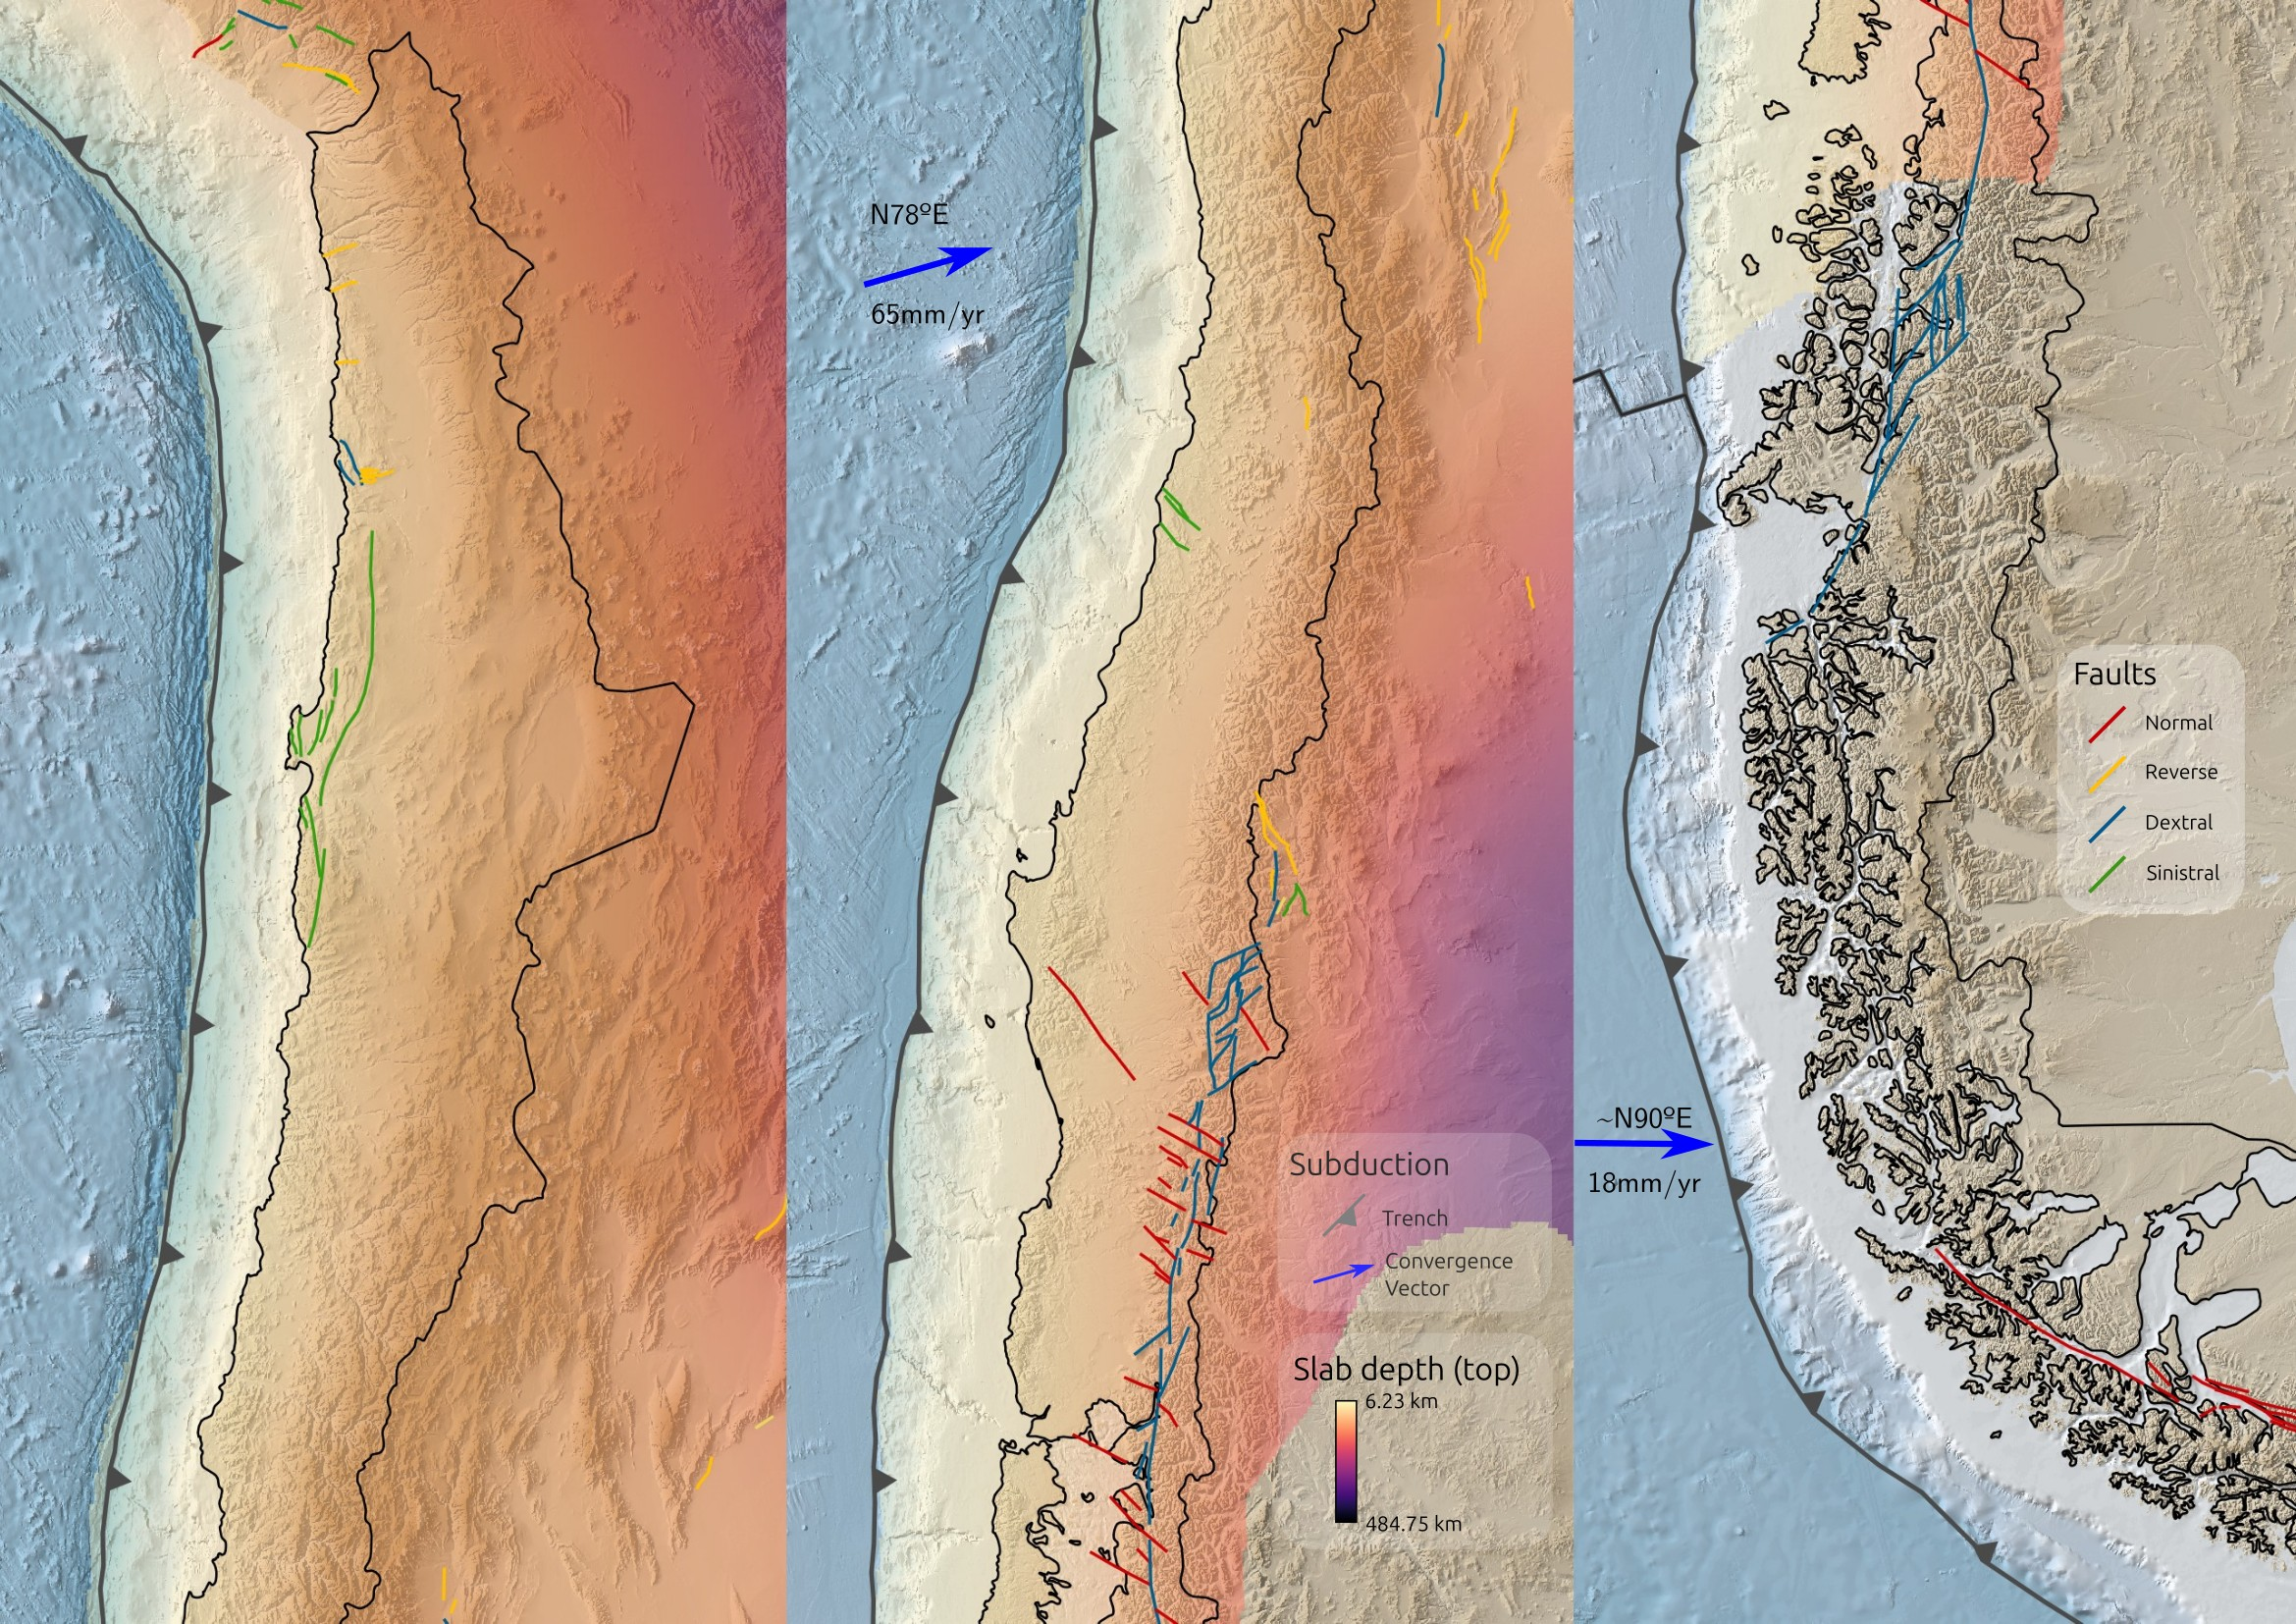
\includegraphics[width=0.6\textwidth]{./figures/faults_sub2}
		\caption*{\scriptsize Compilación armonizada de fallas corticales sudamericanas potencialmente peligrosas (Costa et al., 2020) junto al Slab2 (Hayes, 2018), superficie superior de la subducción.}
	\end{figure}
}
\only<2>{
	\begin{figure}
		\vspace*{-0.2cm}
		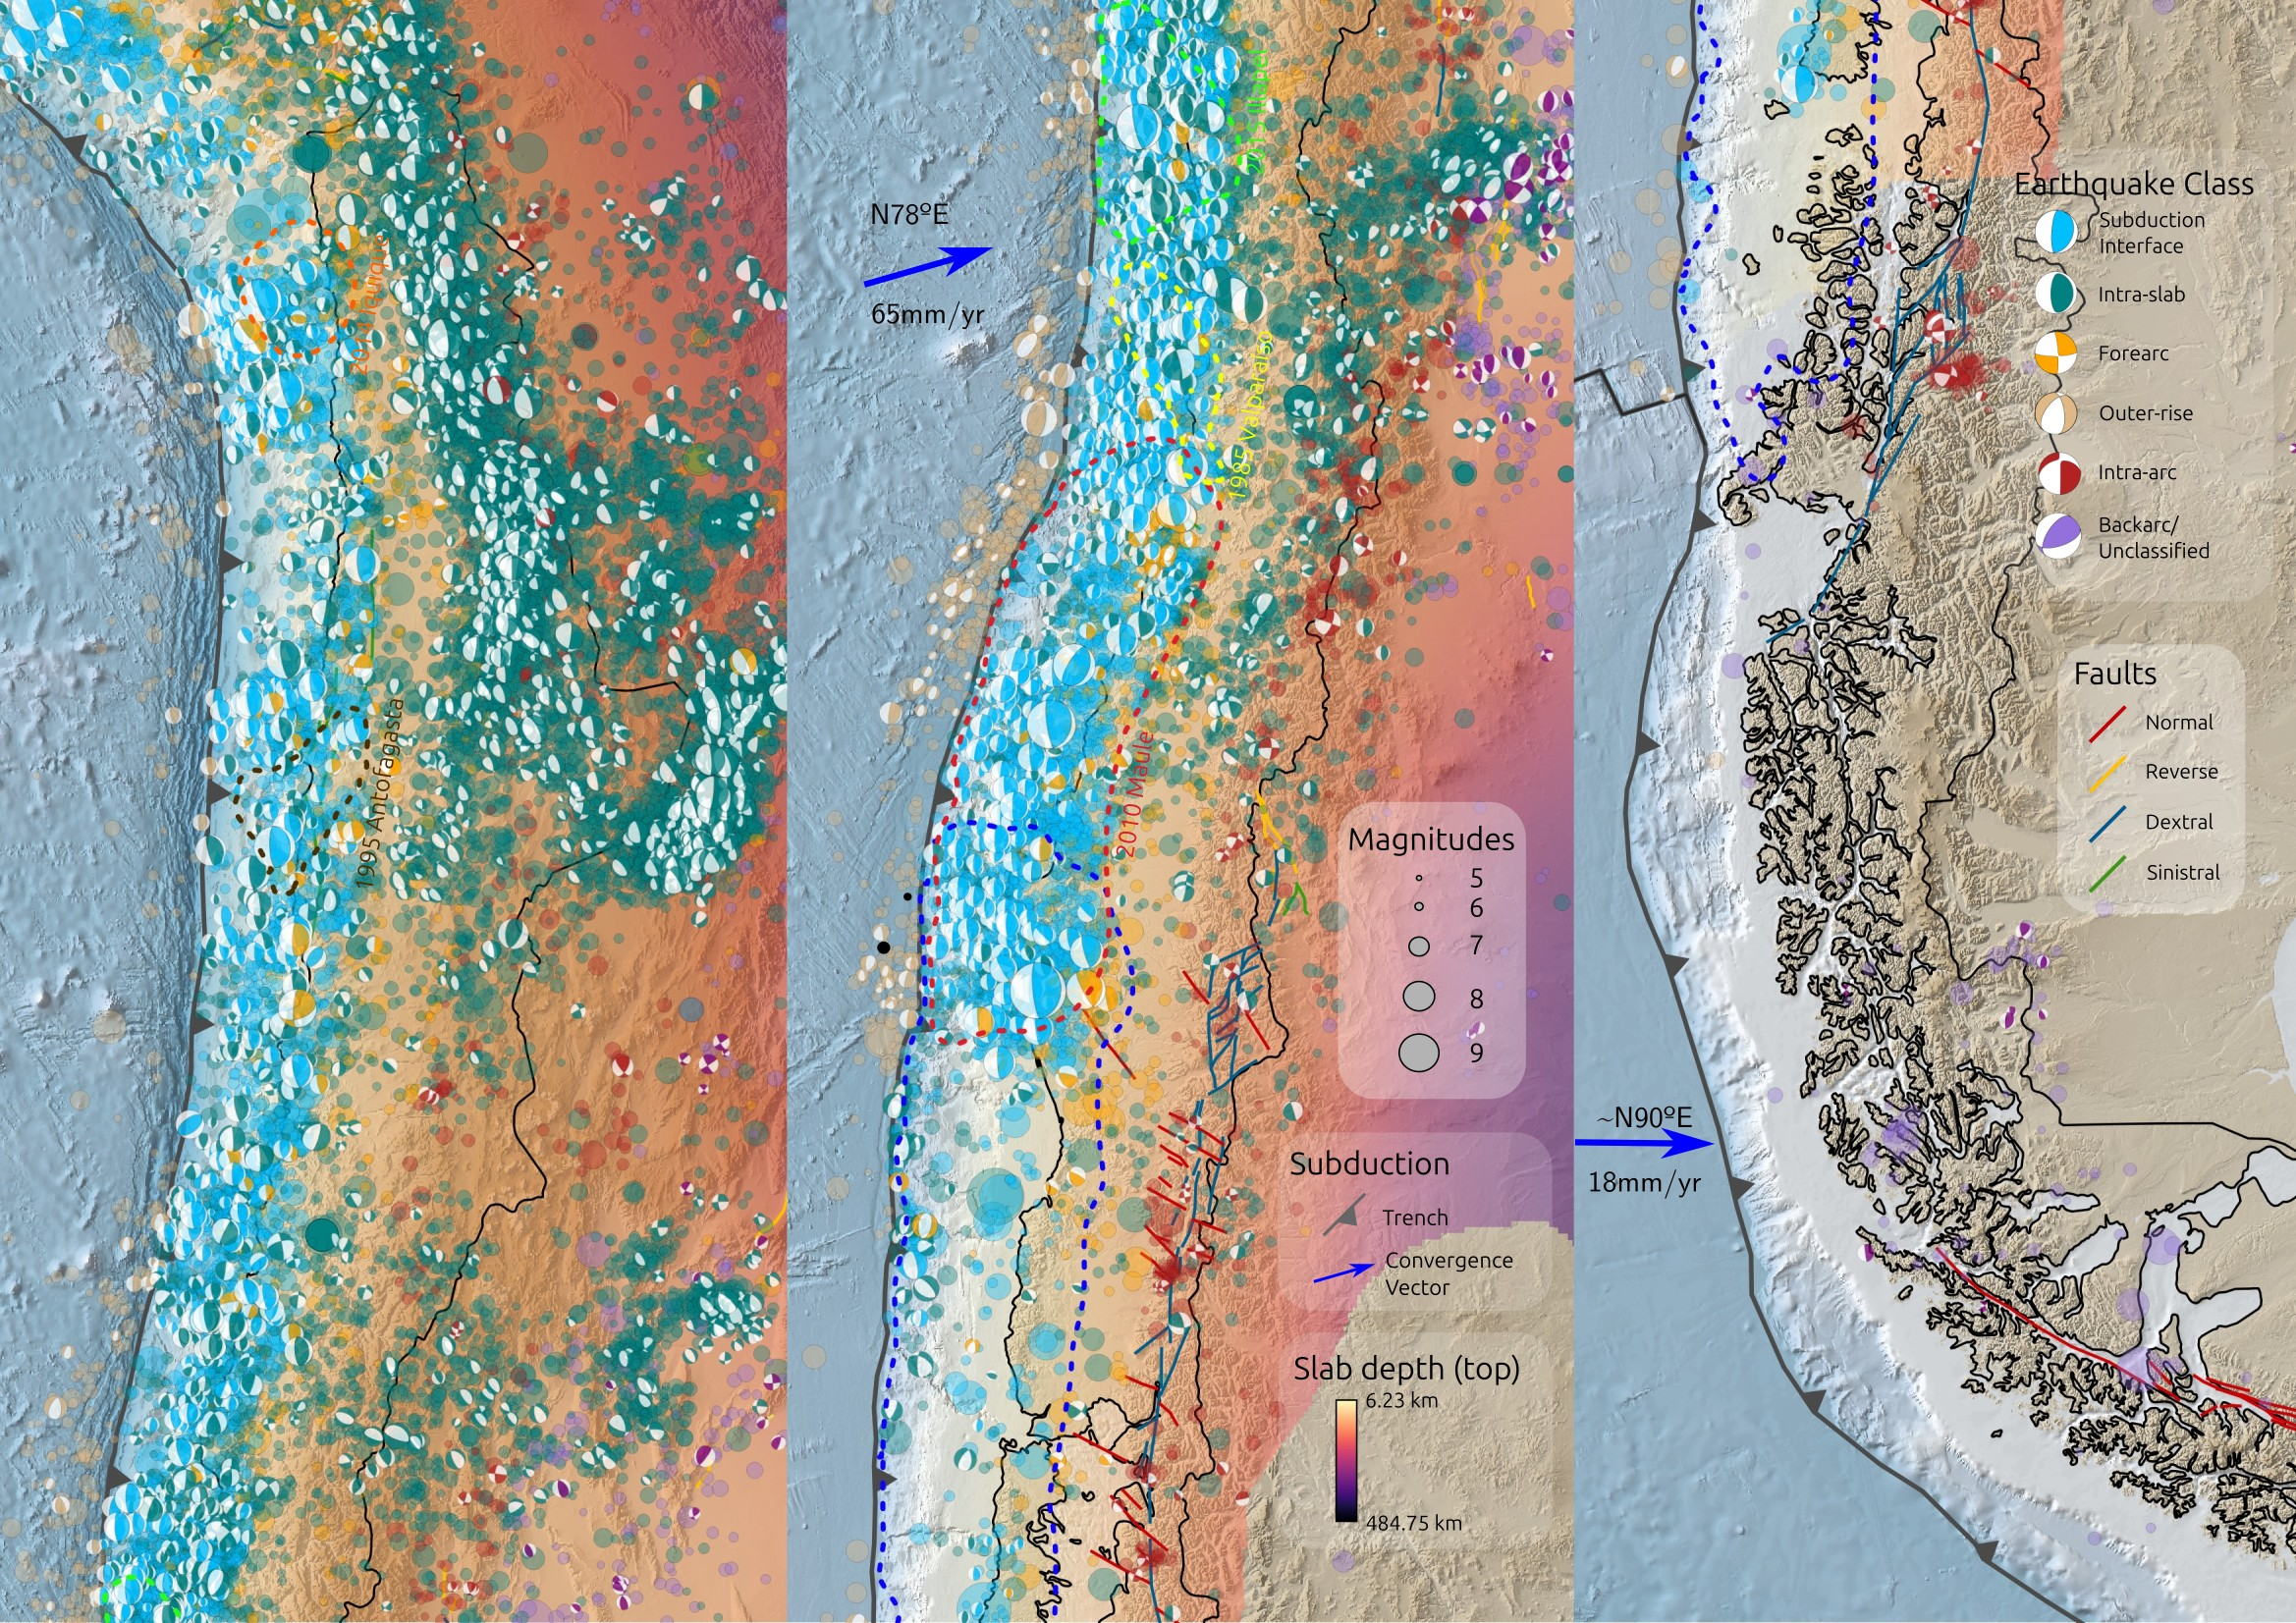
\includegraphics[width=0.6\textwidth]{./figures/fig_full_cat}
		\caption*{\scriptsize Catalog de eventos $M\geq 4.5$ clasificados por régimen tectónico (modificado de Cembrano et al., submitted to Andean Geology, 2025). Data obtenida de Cabello et al., 2025; Potin et al., 2025; Ruiz y Madariaga, 2018; gCMT - Ekström et al., 2012; ANSS, USGS 2017.}
	\end{figure}
}
\end{frame}
%
\begin{frame}[t]
\frametitle{Que es el Análisis de Amenaza Sísmica Probabilistico (PSHA)?}

  Estima la probabilidad de que el movimiento del suelo en un sitio supere un determinado valor de intensidad.\\

\only<2-3>{
\begin{columns}[T,onlytextwidth]
  % LEFT column: text
  \begin{column}{0.65\textwidth}
    \RaggedRight

    \only<2-3>{

			{\vspace{0.2cm}\begin{center} 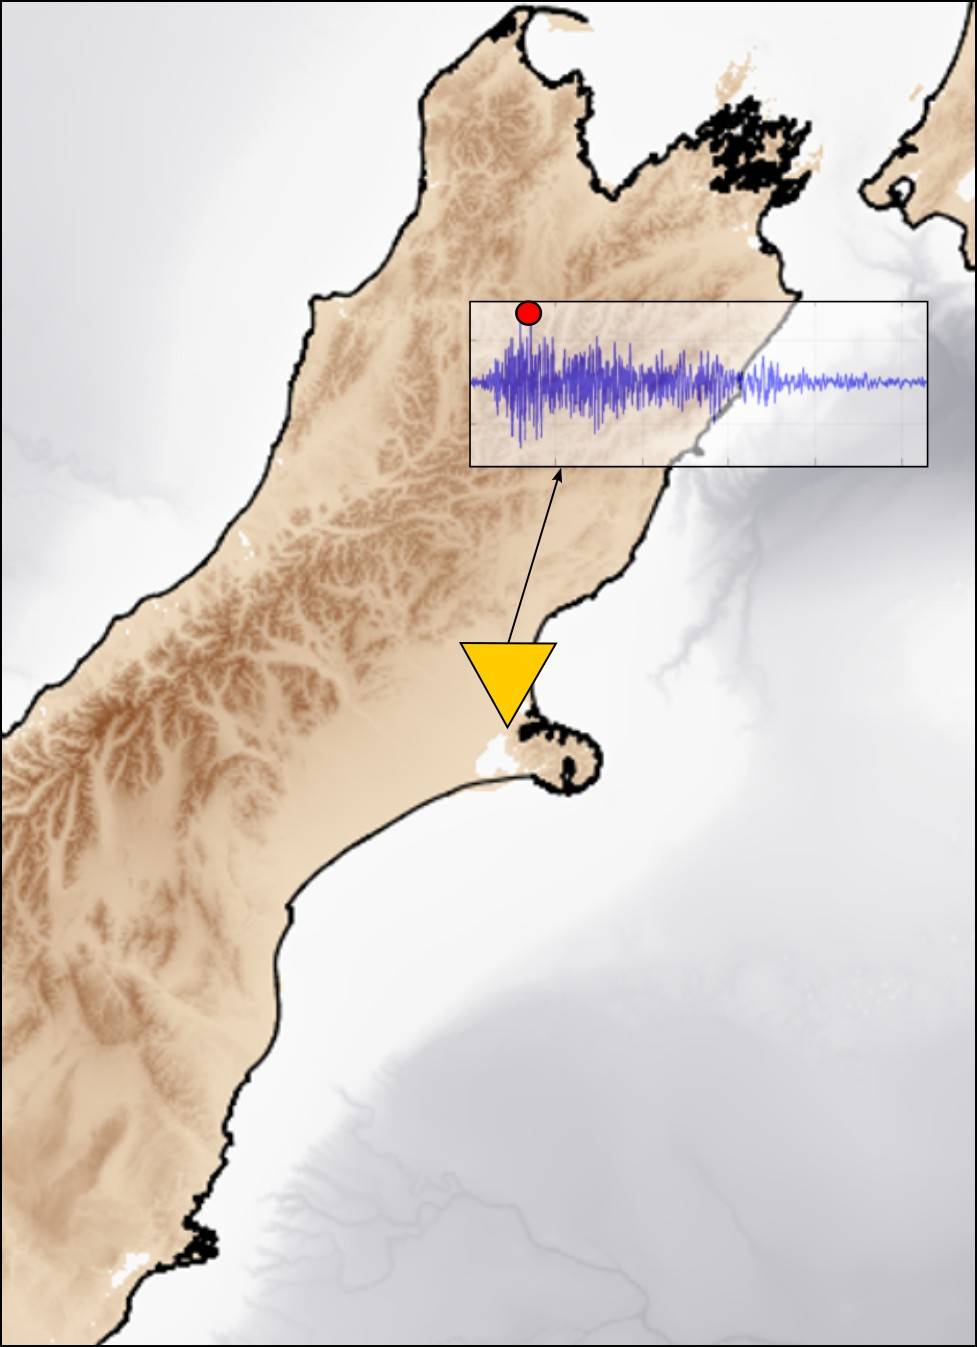
\includegraphics[width=0.4\linewidth]{figures/nz_seism}\end{center}}

    }

  \end{column}

  % RIGHT column: figure (right-aligned)
  \begin{column}{0.35\textwidth}
      \vspace{0.2cm}
    \RaggedLeft
    \only<2>{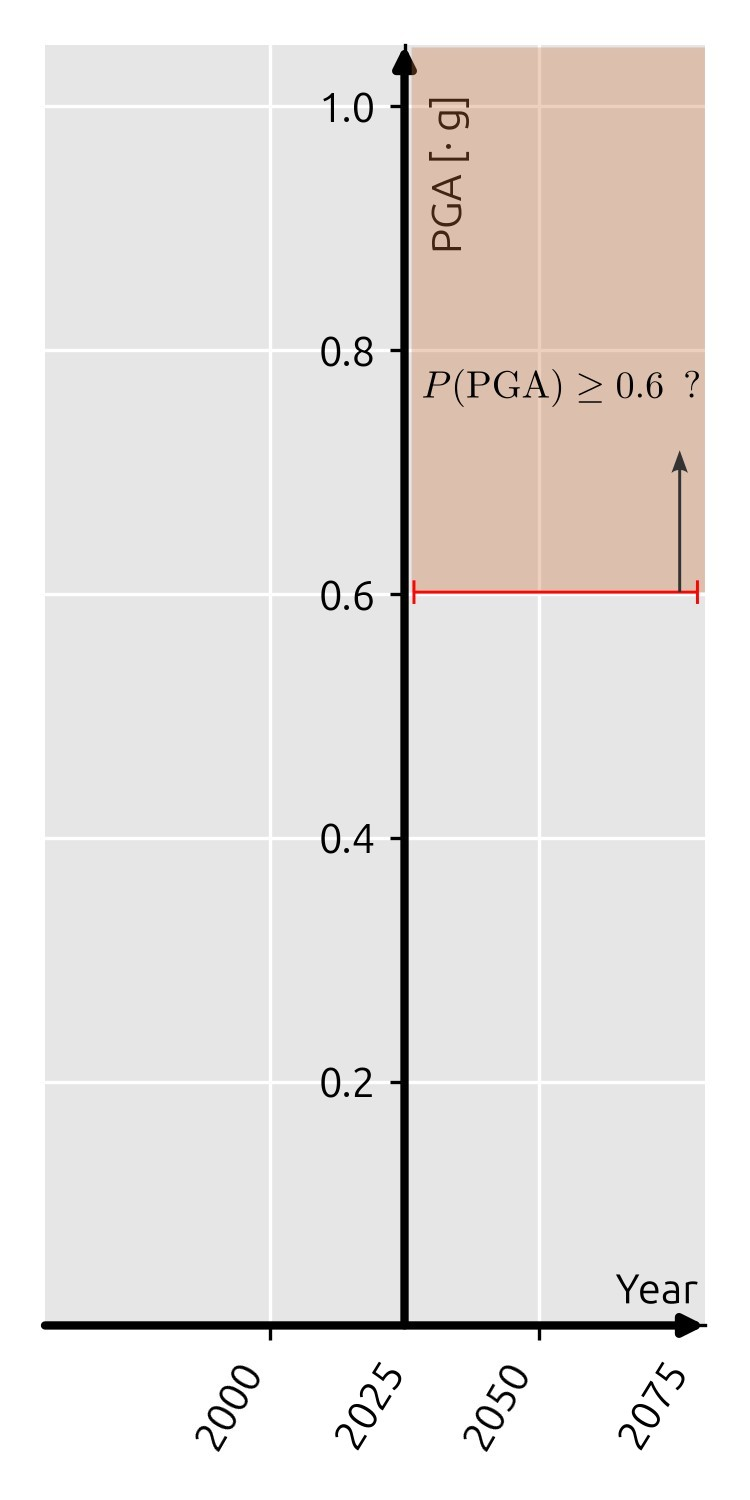
\includegraphics[valign=t,right,max width=0.5\linewidth]{figures/axis}}
    \only<3>{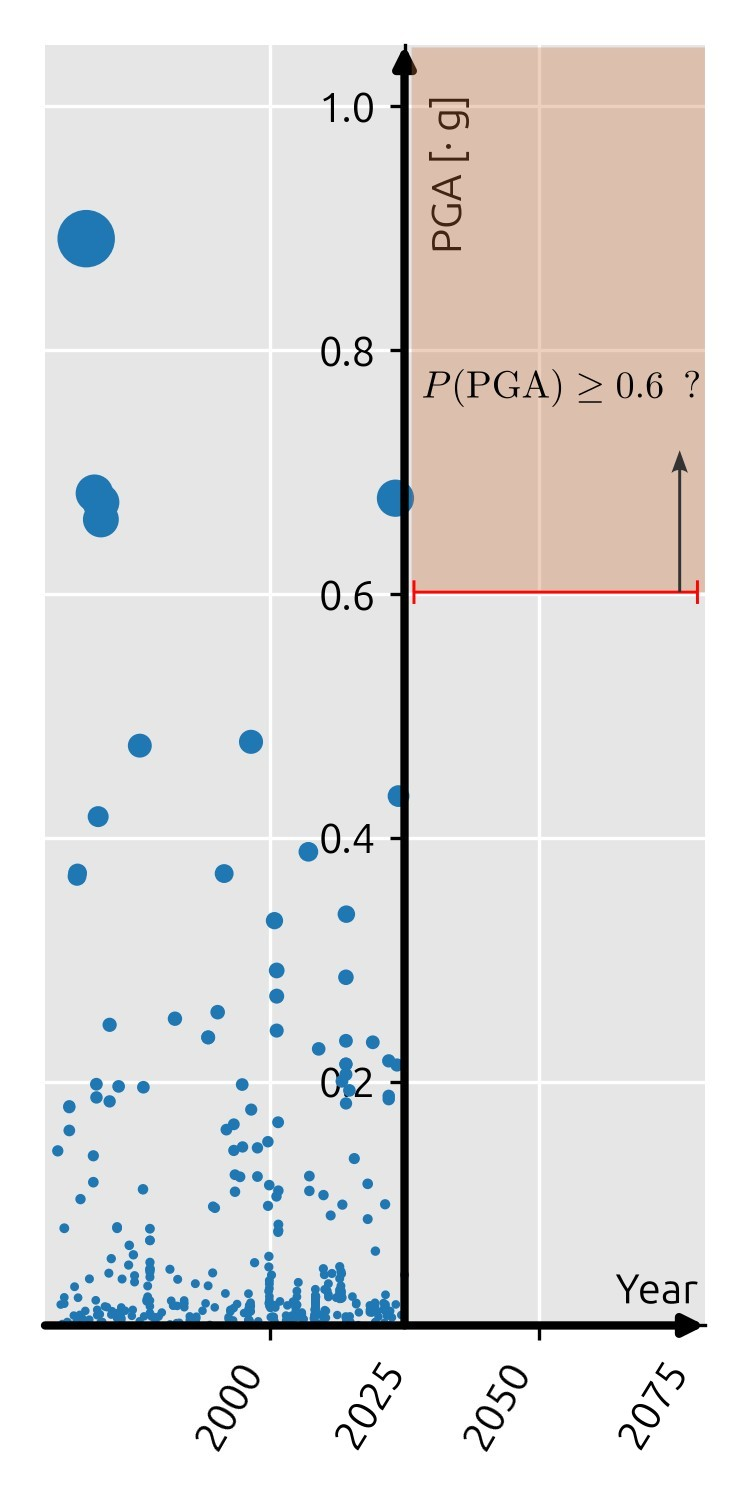
\includegraphics[valign=t,right,max width=0.5\linewidth]{figures/axis2}\hspace{0.1cm}}
  \end{column}
\end{columns}
}

% -------- Overlay 3: figure expands on the RIGHT (takes more space) --------
\only<4>{
\begin{columns}[T,onlytextwidth]
  % LEFT column shrinks
  \begin{column}{0.65\textwidth}
    \RaggedRight

  \end{column}

  % RIGHT column widens; figure right-aligned
  \begin{column}{0.35\textwidth}
      \vspace{0.2cm}
    \RaggedLeft
    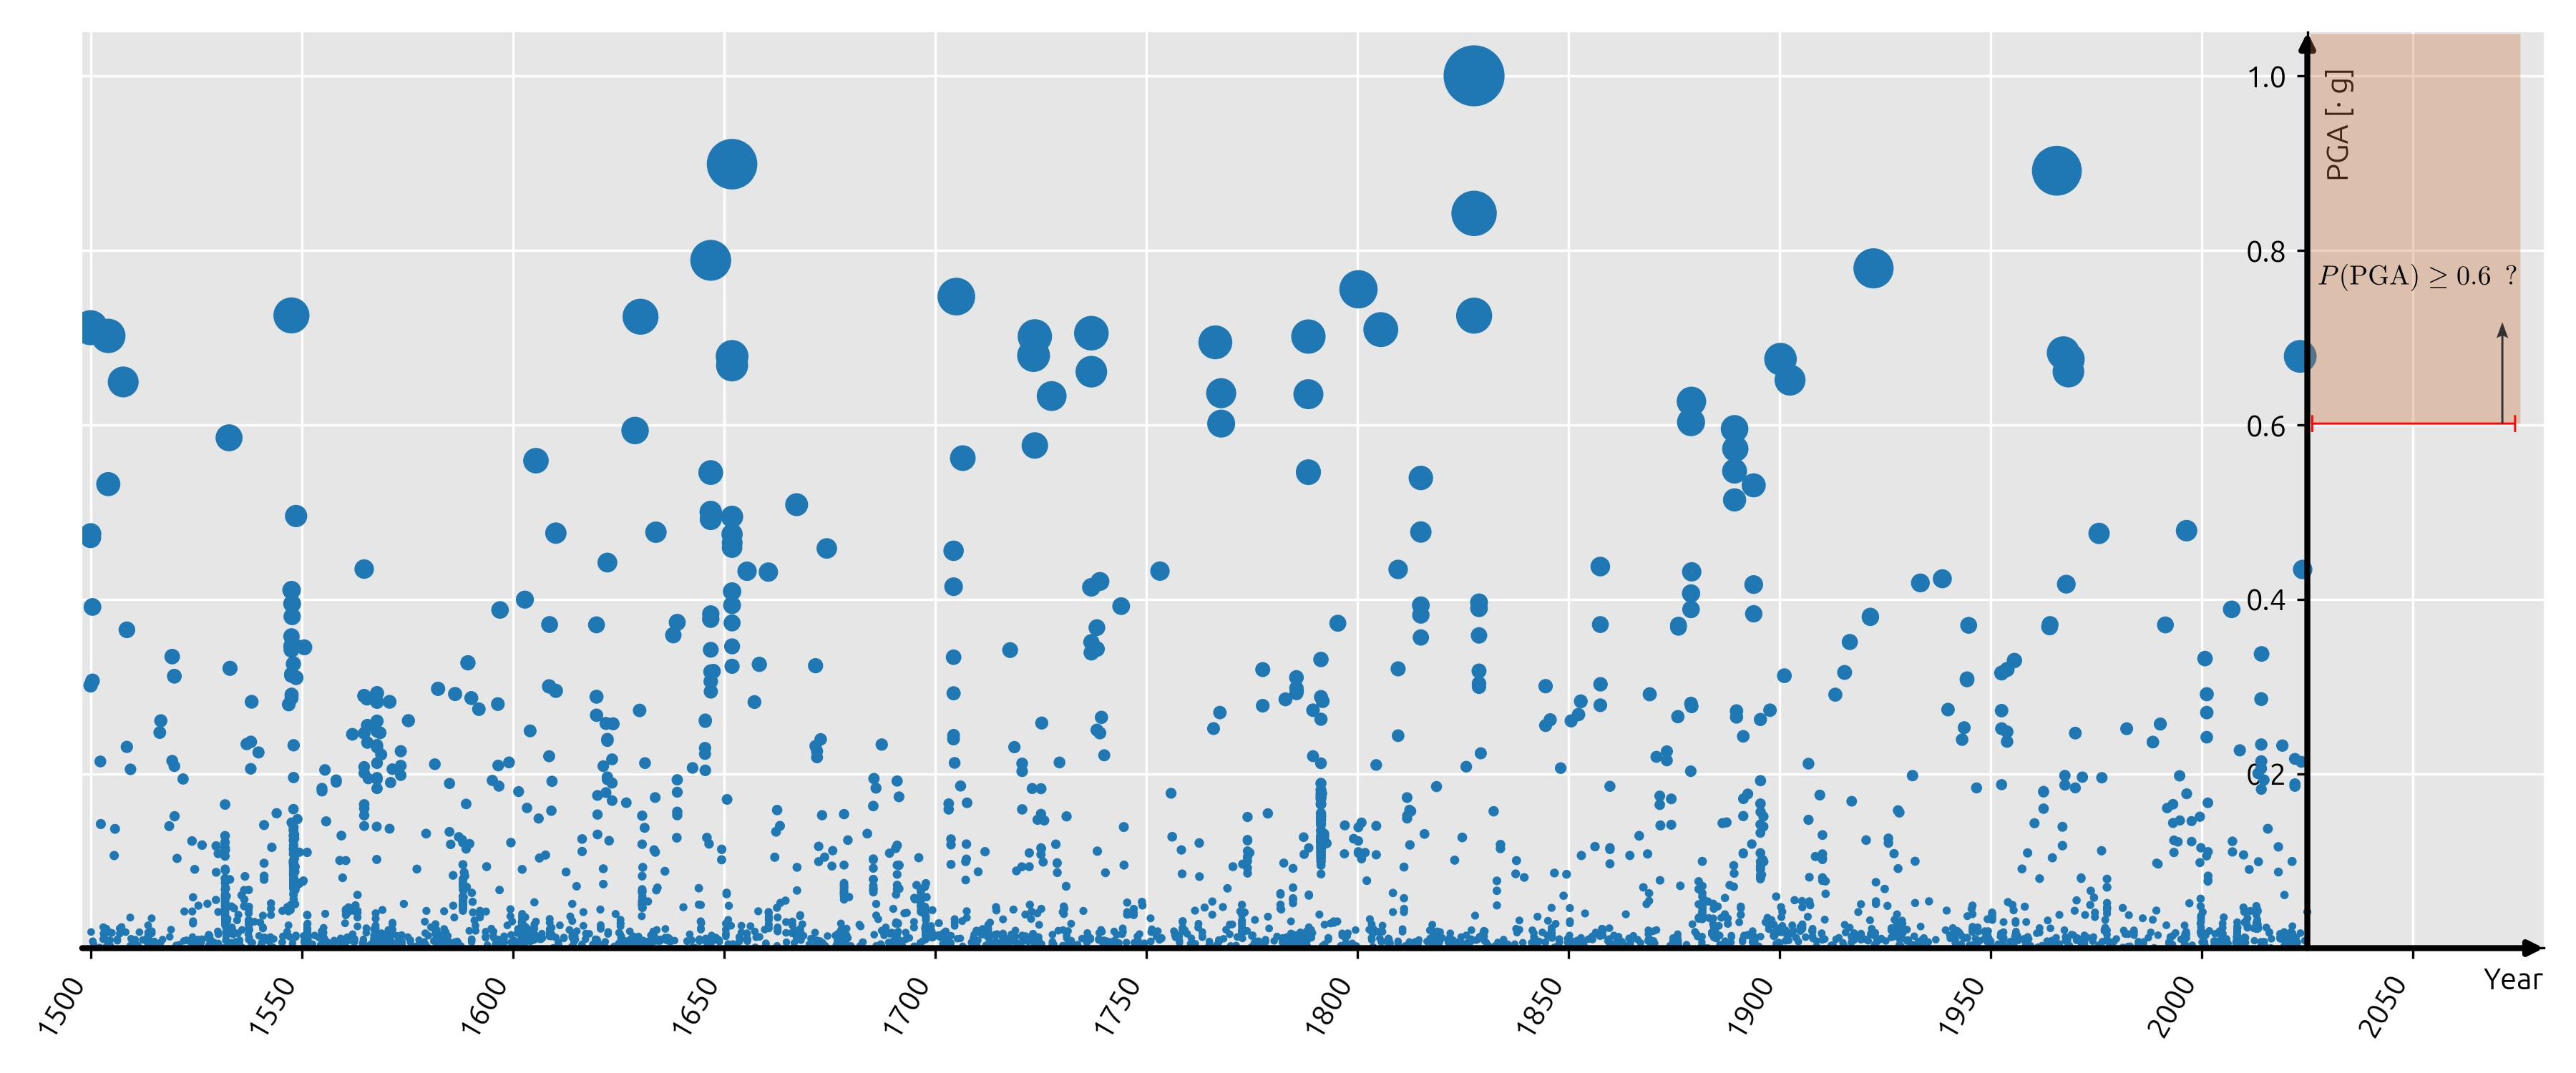
\includegraphics[valign=t,right,max width=0.5\linewidth]{figures/pga_full}
  \end{column}
\end{columns}
}
\only<5>{
\begin{columns}[T,onlytextwidth]
  % LEFT column shrinks
  \begin{column}{0.65\textwidth}
    \RaggedRight
			{\vspace{0.2cm}\begin{center} 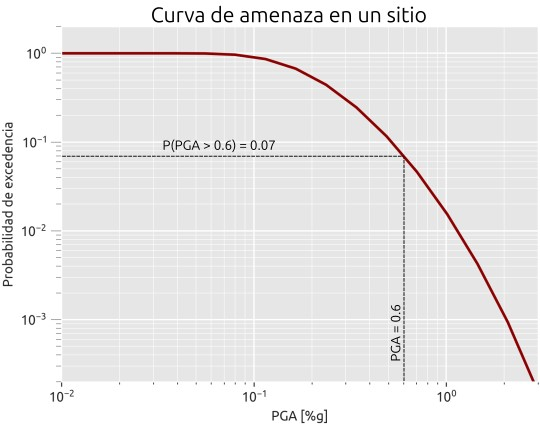
\includegraphics[width=0.8\linewidth]{figures/curva_ejemplo}\end{center}}
  \end{column}

  % RIGHT column widens; figure right-aligned
  \begin{column}{0.35\textwidth}
      \vspace{0.2cm}
    \RaggedLeft
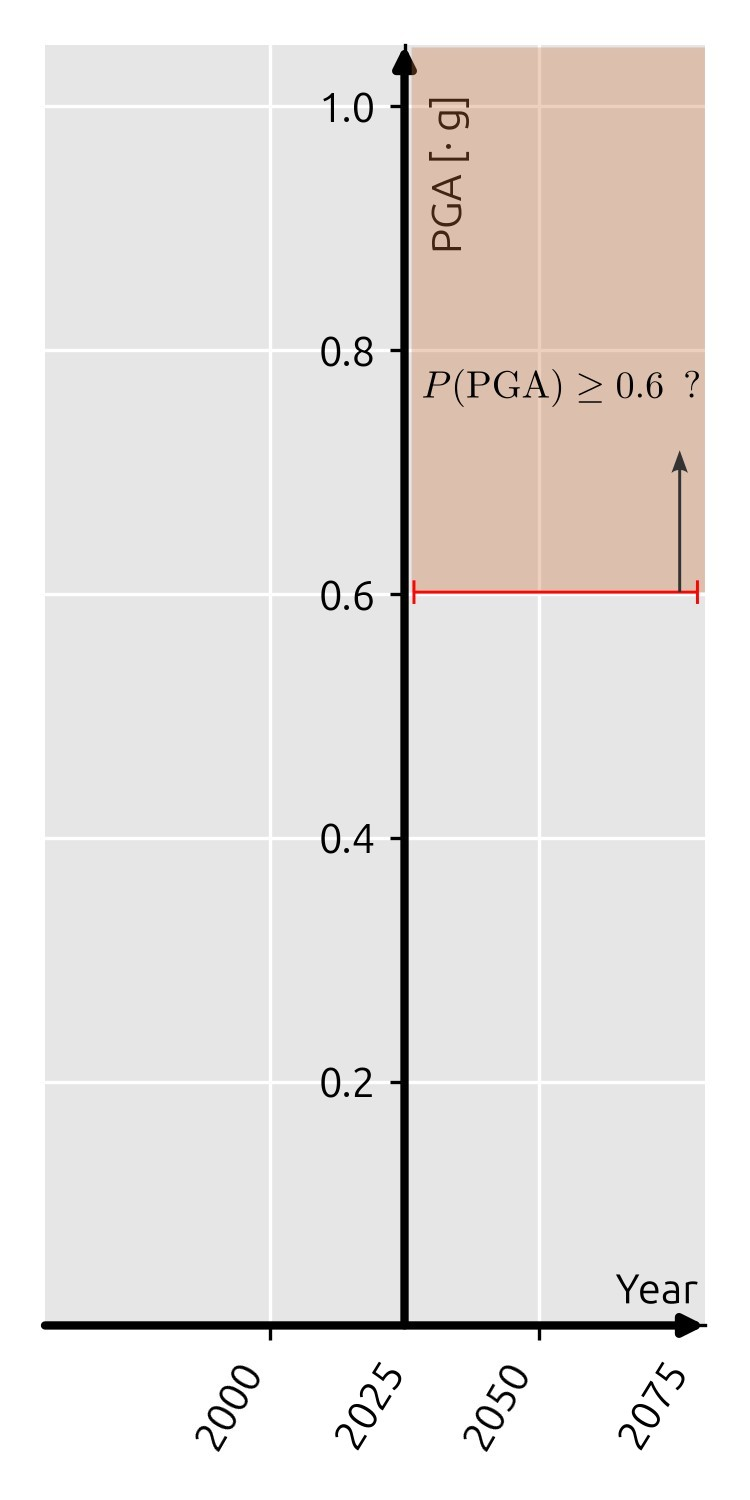
\includegraphics[valign=t,right,max width=0.5\linewidth]{figures/axis}
  \end{column}
\end{columns}
}
\end{frame}
%
%
\begin{frame}[t]
	\frametitle{Como construir un modelo de PSHA}

\begin{columns}[t]

	\column{.55\textwidth}
	\vspace{-0.5cm}
	\only<1-5>{
\begin{itemize}
	\item Combina un modelo de \textbf{occurrencia de terremotos} y un modelo de \textbf{movimiento de suelo}.\\
 \end{itemize}
	}
	\only<2-5>{
	\begin{exampleblock}{\large Earthquake Forecasting (Probabilistico)}

\begin{itemize}
	\item Identifica potenciales fuentes sismogénicas.
	\item Distribuciones espacio-temporales de sismicidad.
	\item Distribuciones de magnitud-frecuencia.
\end{itemize}

	\end{exampleblock}
	\centering

	}
	\only<4-5>{
\begin{alertblock}{\large Modelo de movimiento de suelo (GMM)}
	\begin{itemize}
\item Intensidad de movimiento para un sitio(s) como functión de las características del terremoto y condiciones del suelo.
\end{itemize}
	\end{alertblock}
	}
	\only<6>{
		\begin{figure}

		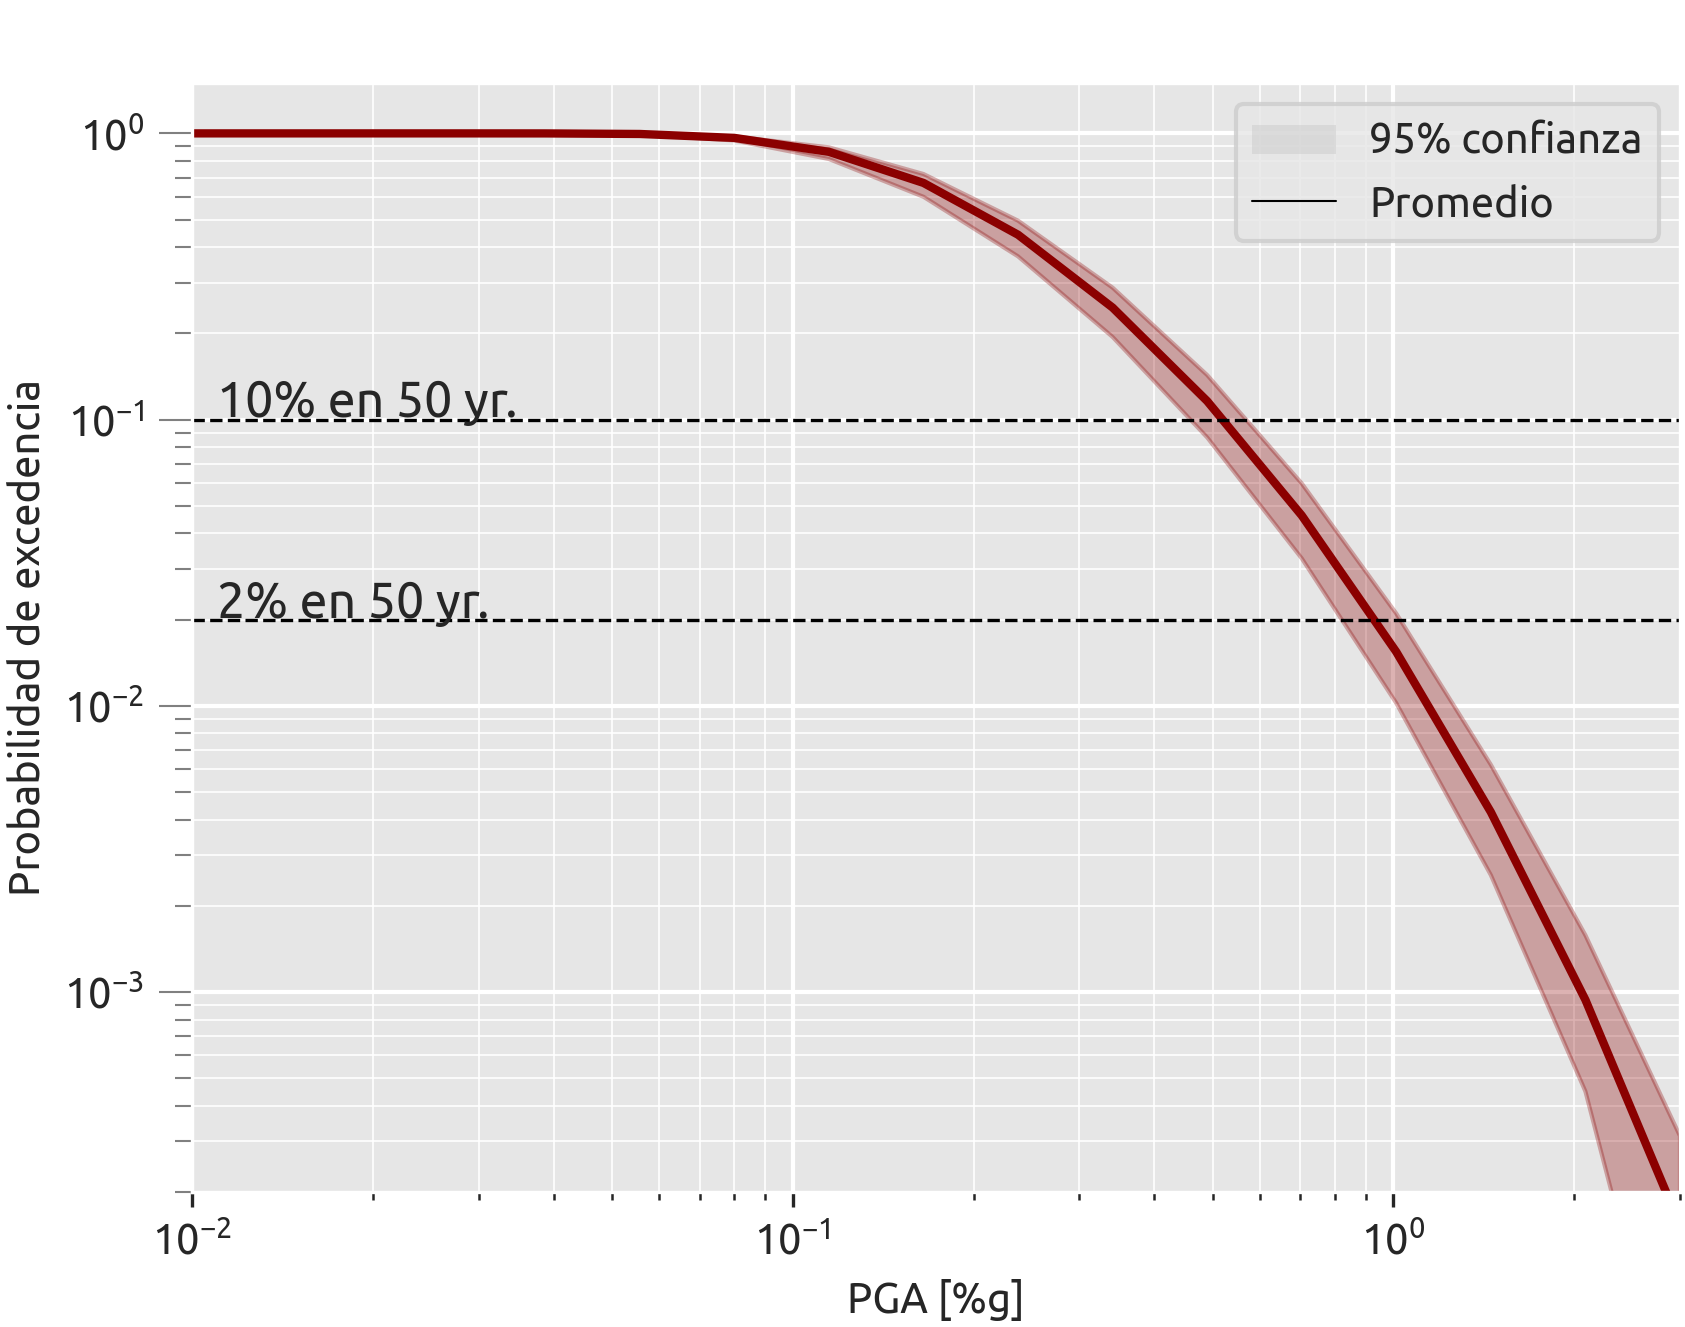
\includegraphics[width=0.85\textwidth]{./figures/curva_2}
		\caption*{\scriptsize Curva de amenaza}
	\end{figure}
	}
	\column{.45\textwidth}

	\only<2>{
		\begin{figure}
		\vspace*{-0.5cm}
		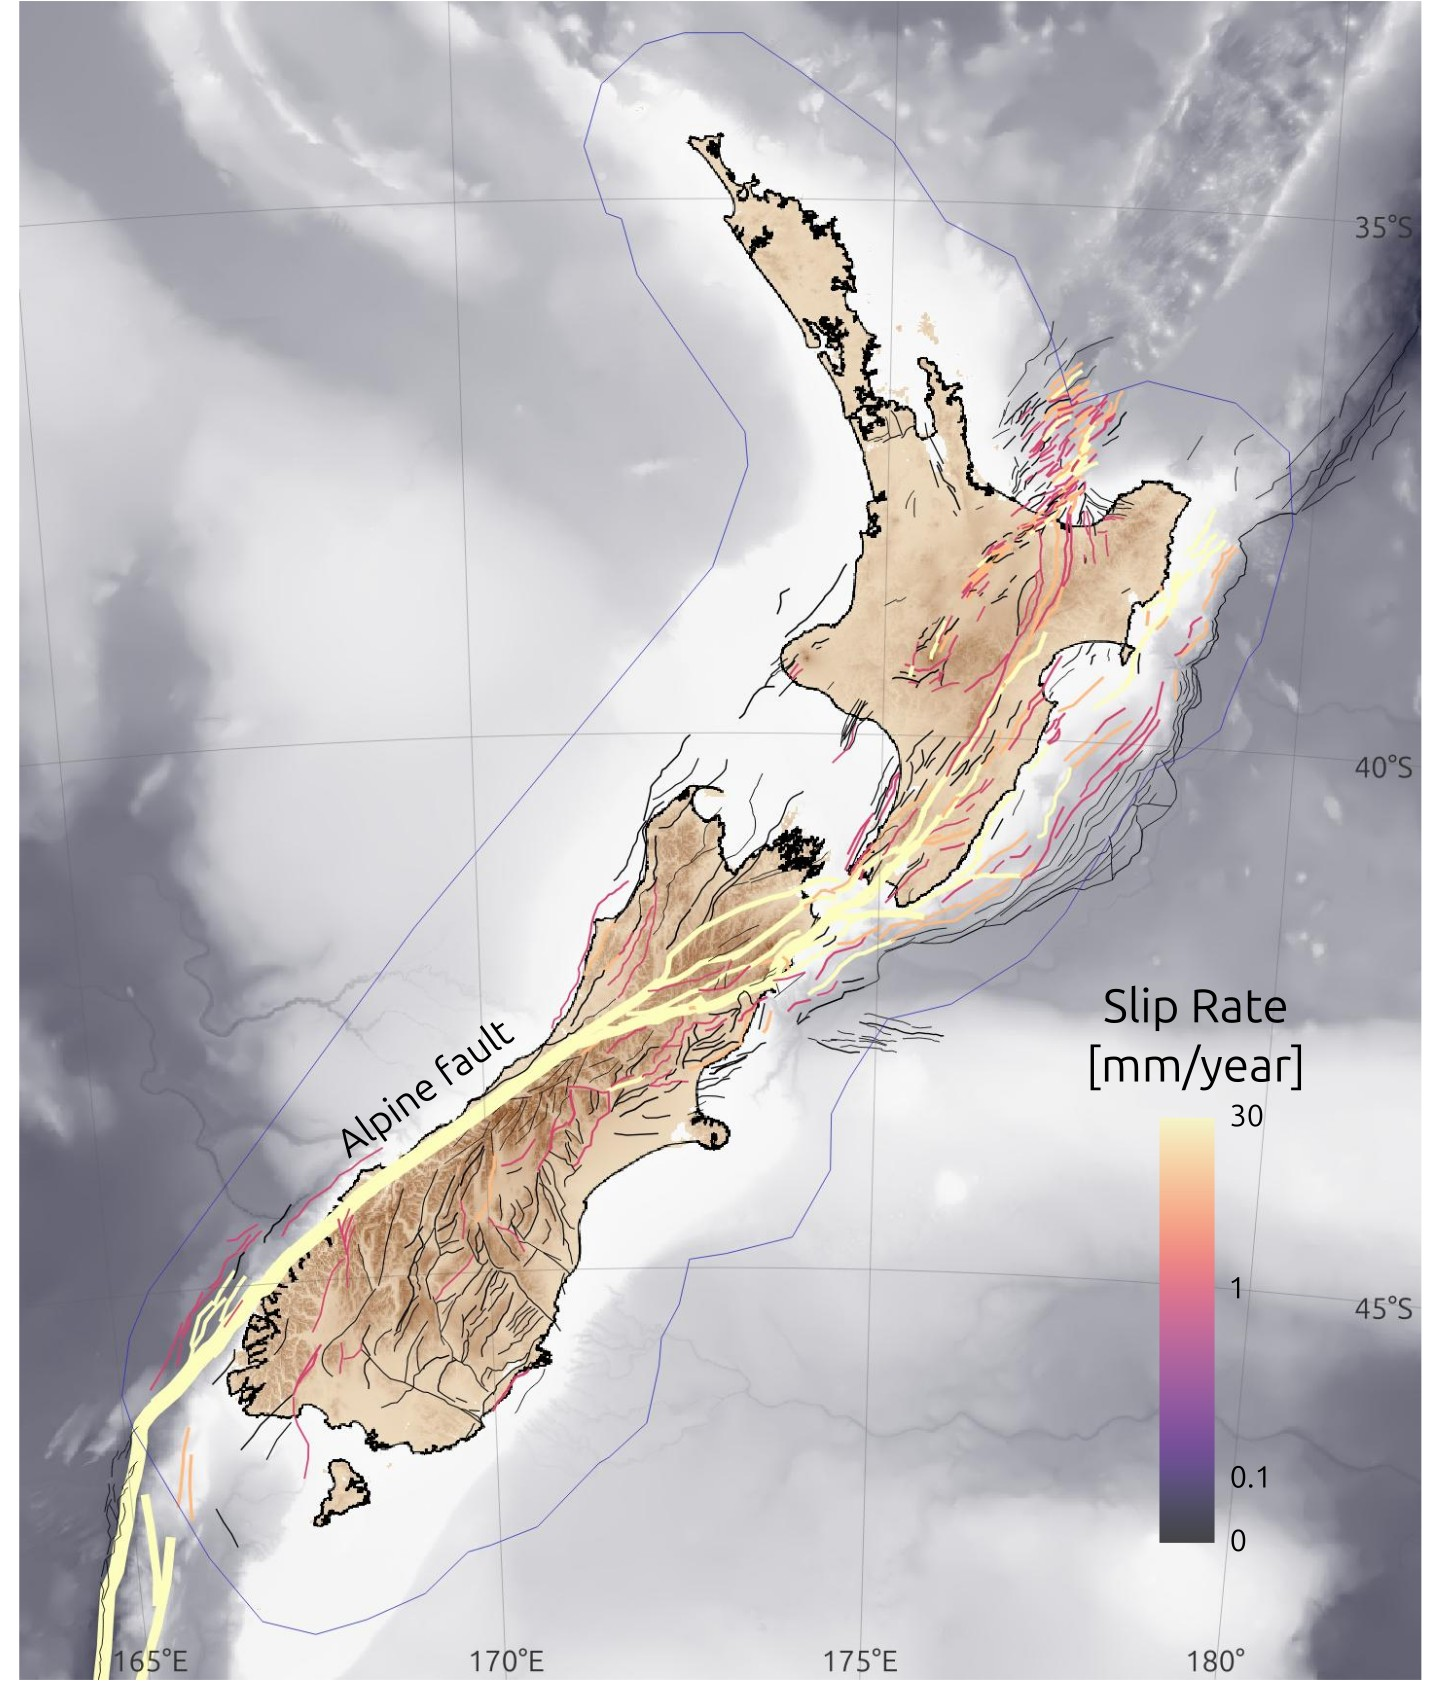
\includegraphics[width=0.85\textwidth]{./figures/faults_map}
		\caption*{\scriptsize Community Fault Model - Fallas corticales de Nueva Zelanda (Seebeck et al., 2025)}
	\end{figure}
	}
	\only<3>{
		\begin{figure}
		\vspace*{-0.5cm}
		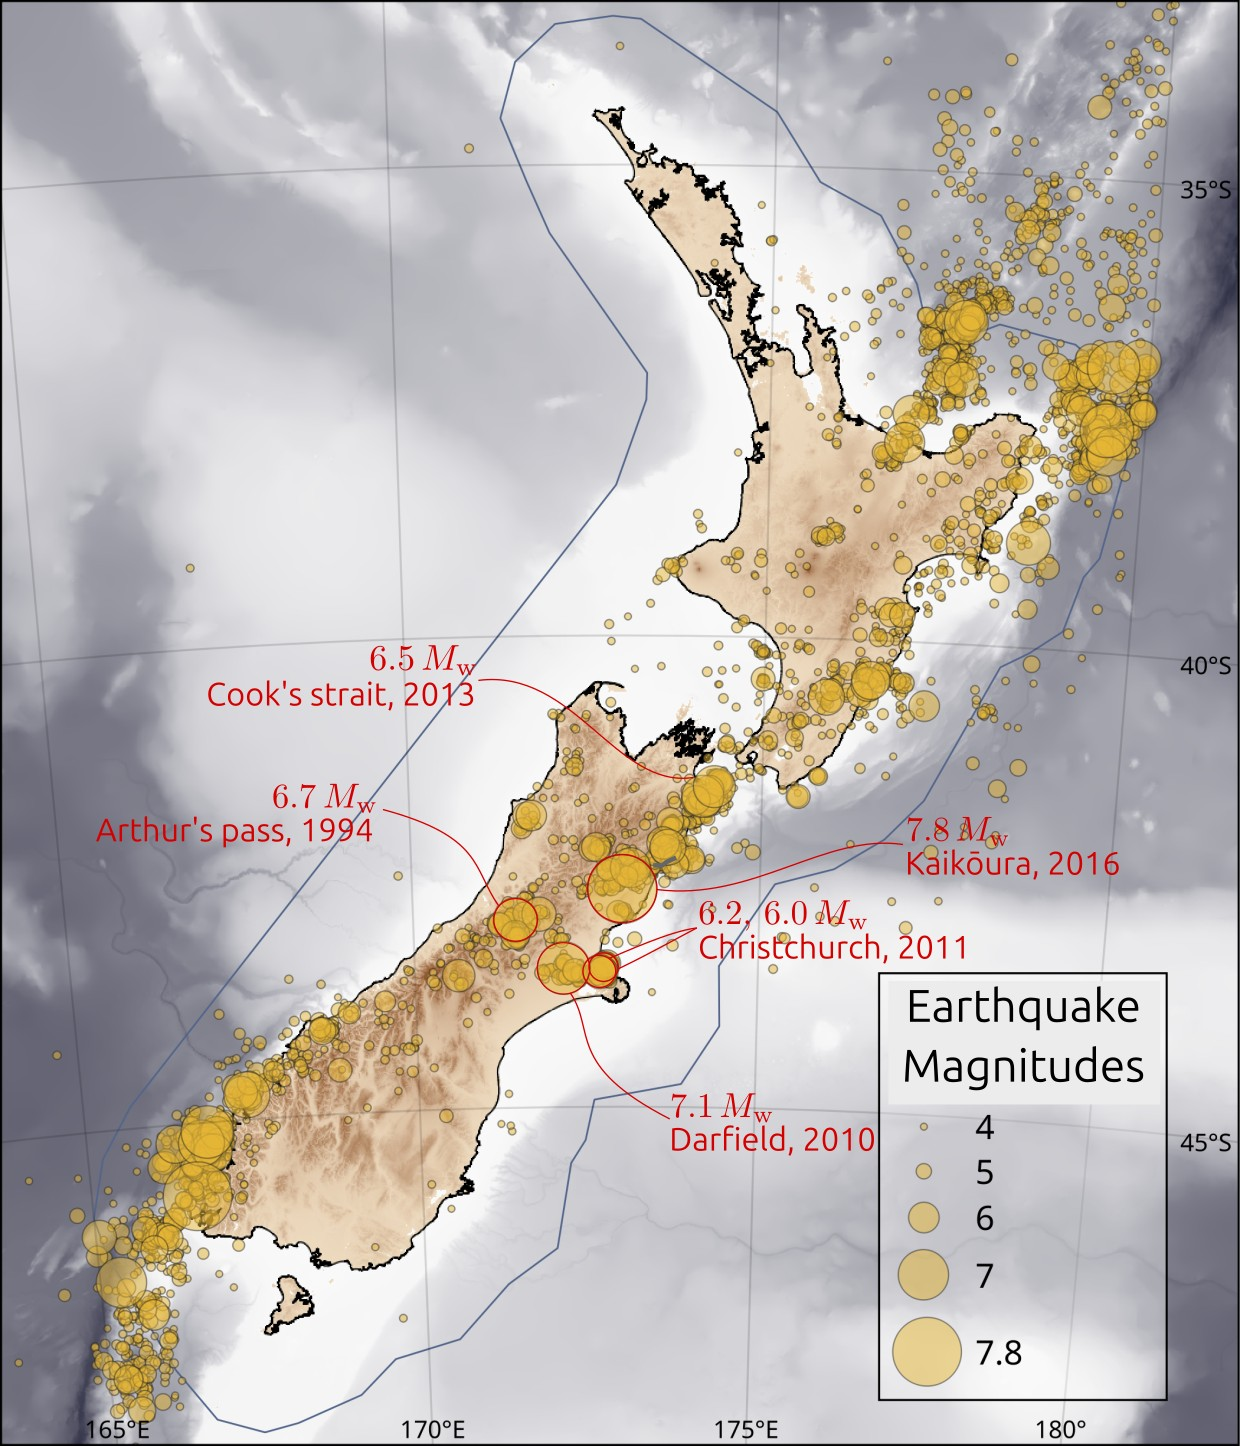
\includegraphics[width=0.85\textwidth]{./figures/catalog_nz}
		\caption*{\scriptsize Sismicidad desde 1964 (Christophersen et al., 2022)}
	\end{figure}
	}
	\only<5-6>{
	\begin{figure}
		\vspace*{-1.cm}
		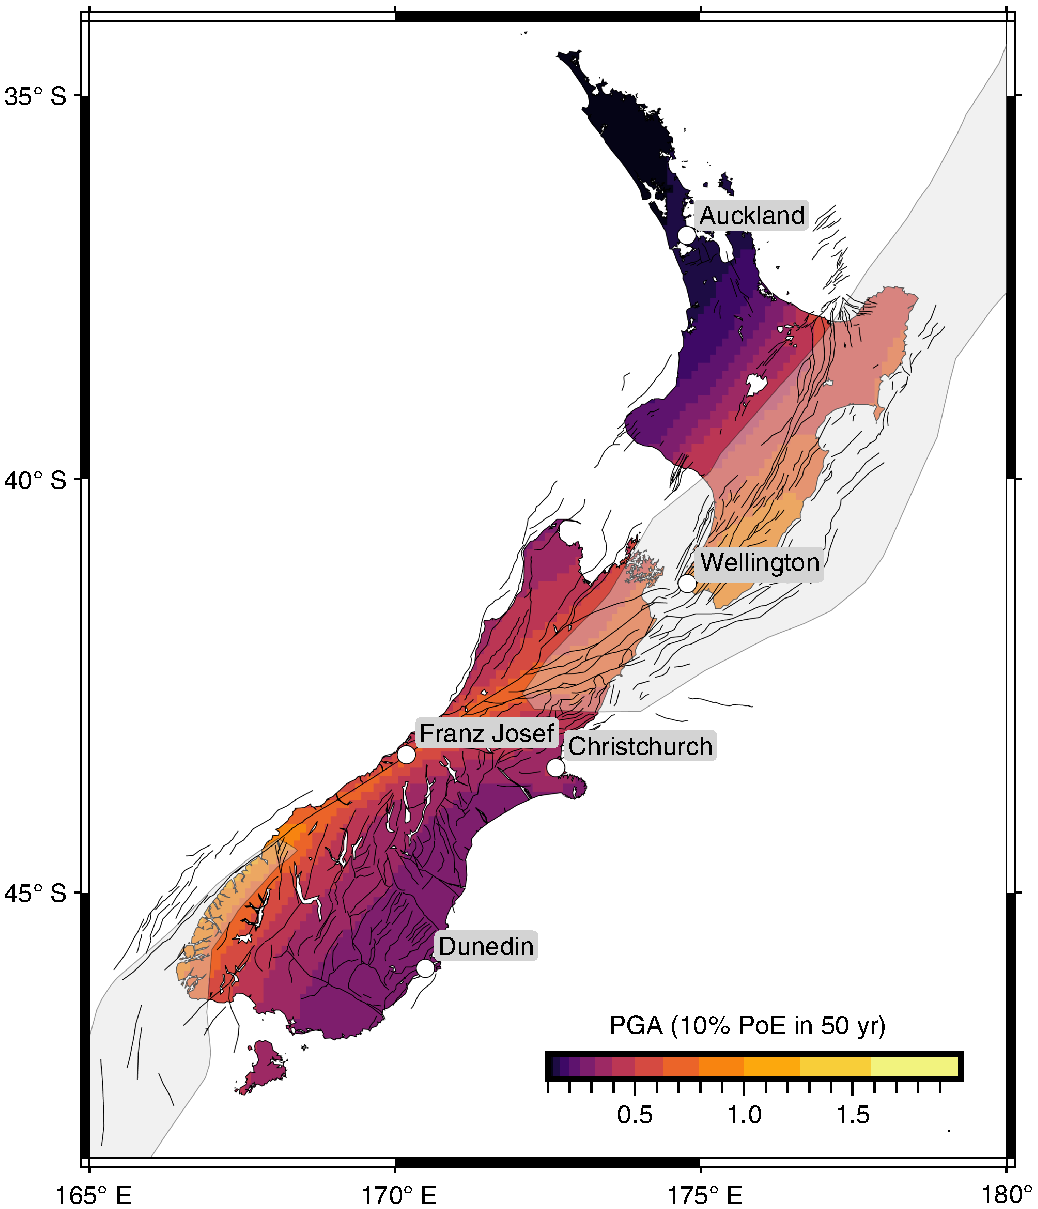
\includegraphics[width=0.85\textwidth]{./figures/hazard_model_nz}
		\caption*{\scriptsize Modelo de amenaza sísmica de Nueva Zelanda, 2022 (Gerstenberger et al., 2023). PGA con un 10\% de probablidad de ser excedido al menos una vez en 50 years ($V_{\mathrm{S}30}=250 \, \mathrm{m}/\mathrm{s}$).}
	\end{figure}
	}
\end{columns}

\end{frame}


\begin{frame}[t]
\frametitle{Construcción de un modelo de PSHA para Chile}


Para cuantificar el rol de las fallas en la amenaza, es necesario ver el efecto conjugado con todas las fuentes sísmicas probabilísticamente.

\begin{columns}[t]
		\column{.45\textwidth}

		\begin{itemize}\small
		\item Interfaz Subducción
		\item Subducción Intraplaca
		\item Sismicidad Cortical - Antearco (*)
		\item Sismicidad Cortical - Intra-arco (*)
		\end{itemize}
			\begin{figure}

			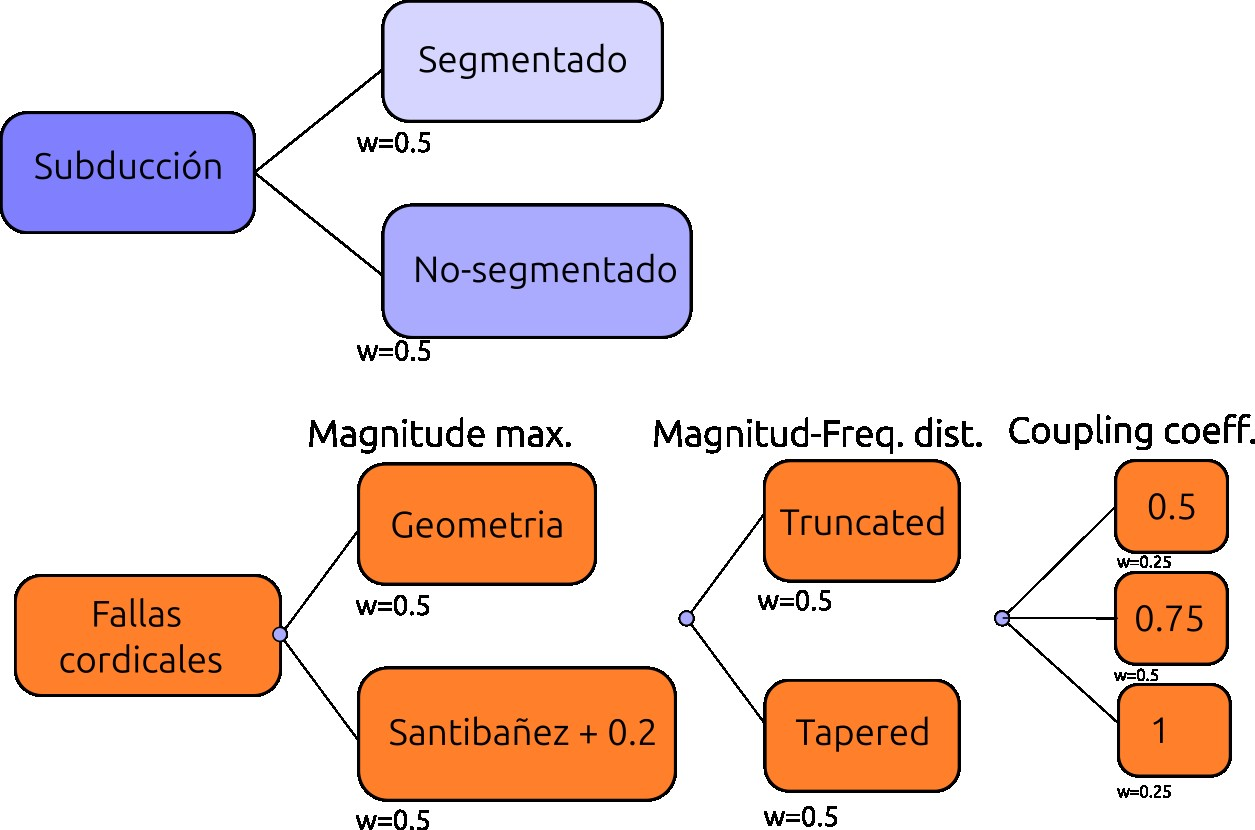
\includegraphics[width=0.75\textwidth]{./figures/logic}
				\caption*{Logic-tree para caracterizar incertidumbre epistémica.}
			\end{figure}
		\column{.55\textwidth}

		\begin{figure}
		\vspace*{-0.6cm}
		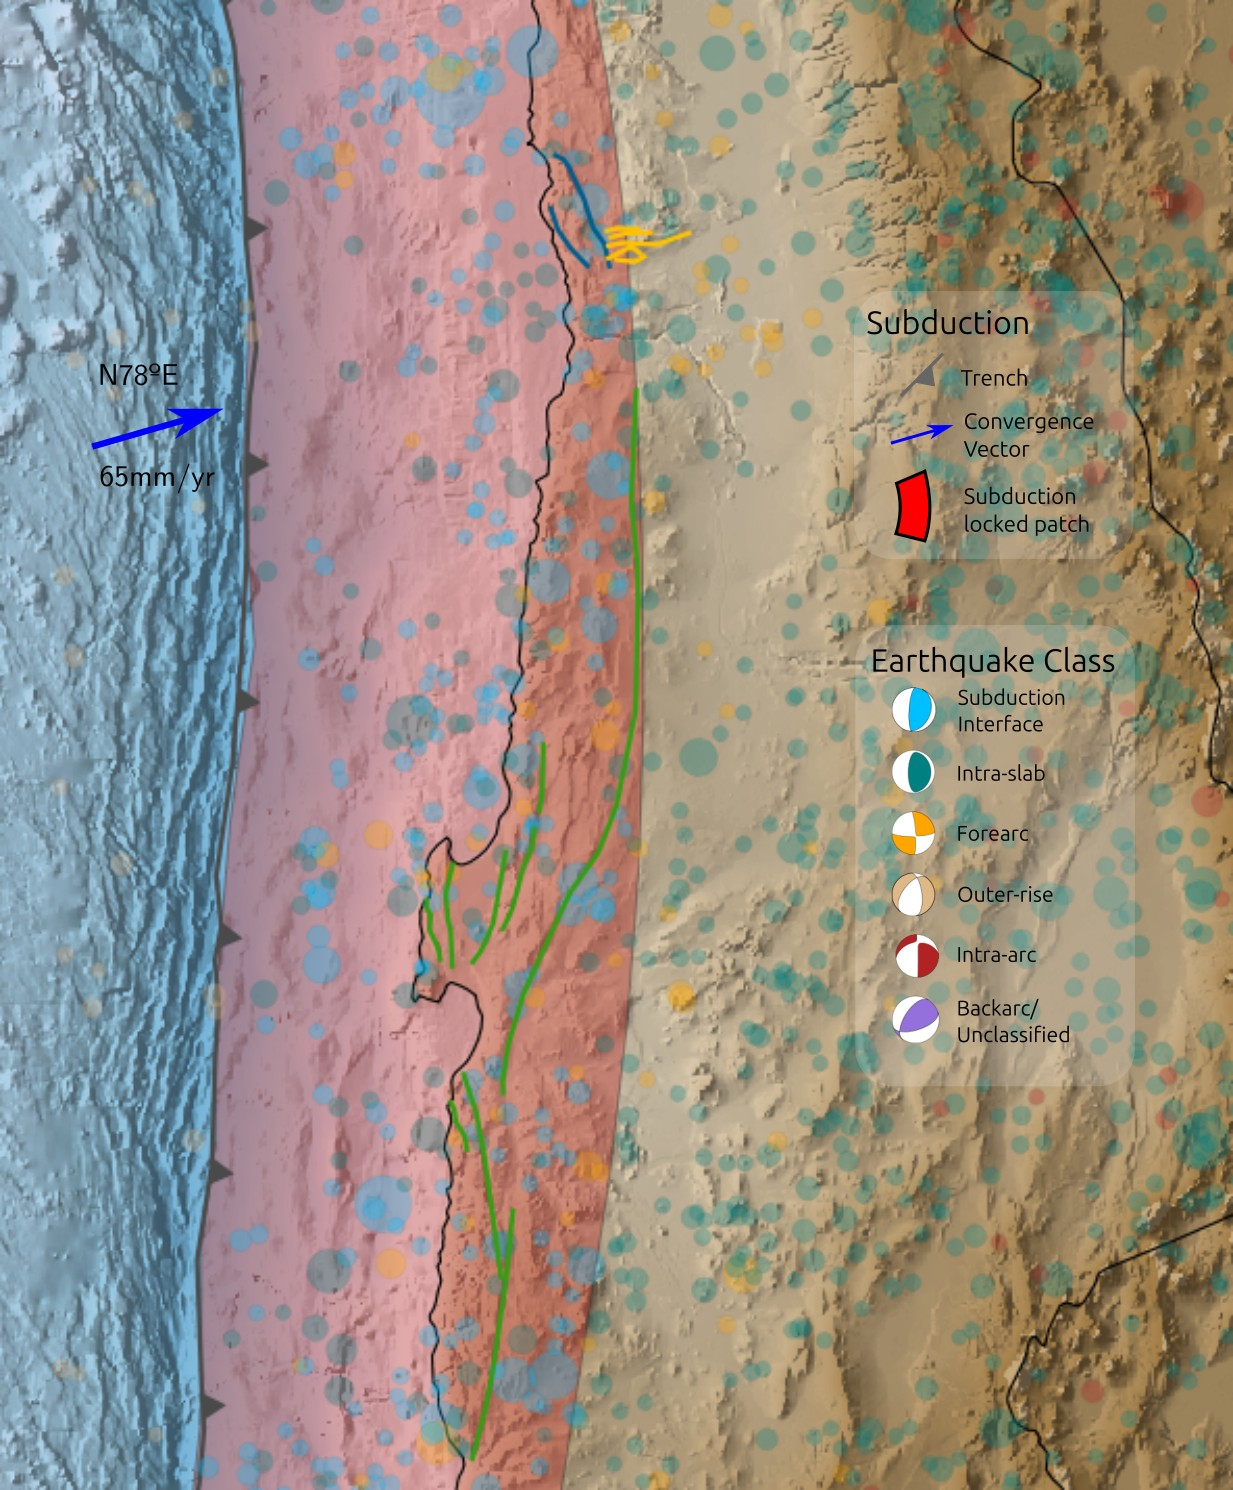
\includegraphics[width=0.65\textwidth]{./figures/fuentes}
		\end{figure}
\end{columns}

\end{frame}



\begin{frame}[t]
	Supuestos y/o procesamiento de datos:


	\begin{itemize}\small
		\item Estacionariedad y terremotos independientes sin memoria - Poisson (*)
		\item Uso de logic-tree para caracterizar incertidumbre epistémica (*)
		\item GMM ergódicos usados en Nueva Zelanda (Bradley et al., 2024) y Europa (Danciu et al., 2024)
		\item Clasificación de catálogo por régimen tectónico (Rollins et al., 2025).
		\item Distribución de profundidad / mecanismos focales (Rollins et al., 2025, von Specht et al., 2017).
		\item Geometría interfaz de subducción bloqueada bloqueada (50 km).
		\item Segmentación de la subducción (*).
		\item Magnitud de completitud por ventana de tiempo (Mizrahi et al., 2024, Van der Elst, 2023).
		\item Declustering (Gartner and Knopoff, 1974; Zaliapin et al., 2008).
		\item Magnitud máxima (*).
		\item Gutenberg-Richter a-b values fit (Kijko and Smit, 2015).
	\end{itemize}

		\begin{figure}
		\vspace*{-0.2cm}
		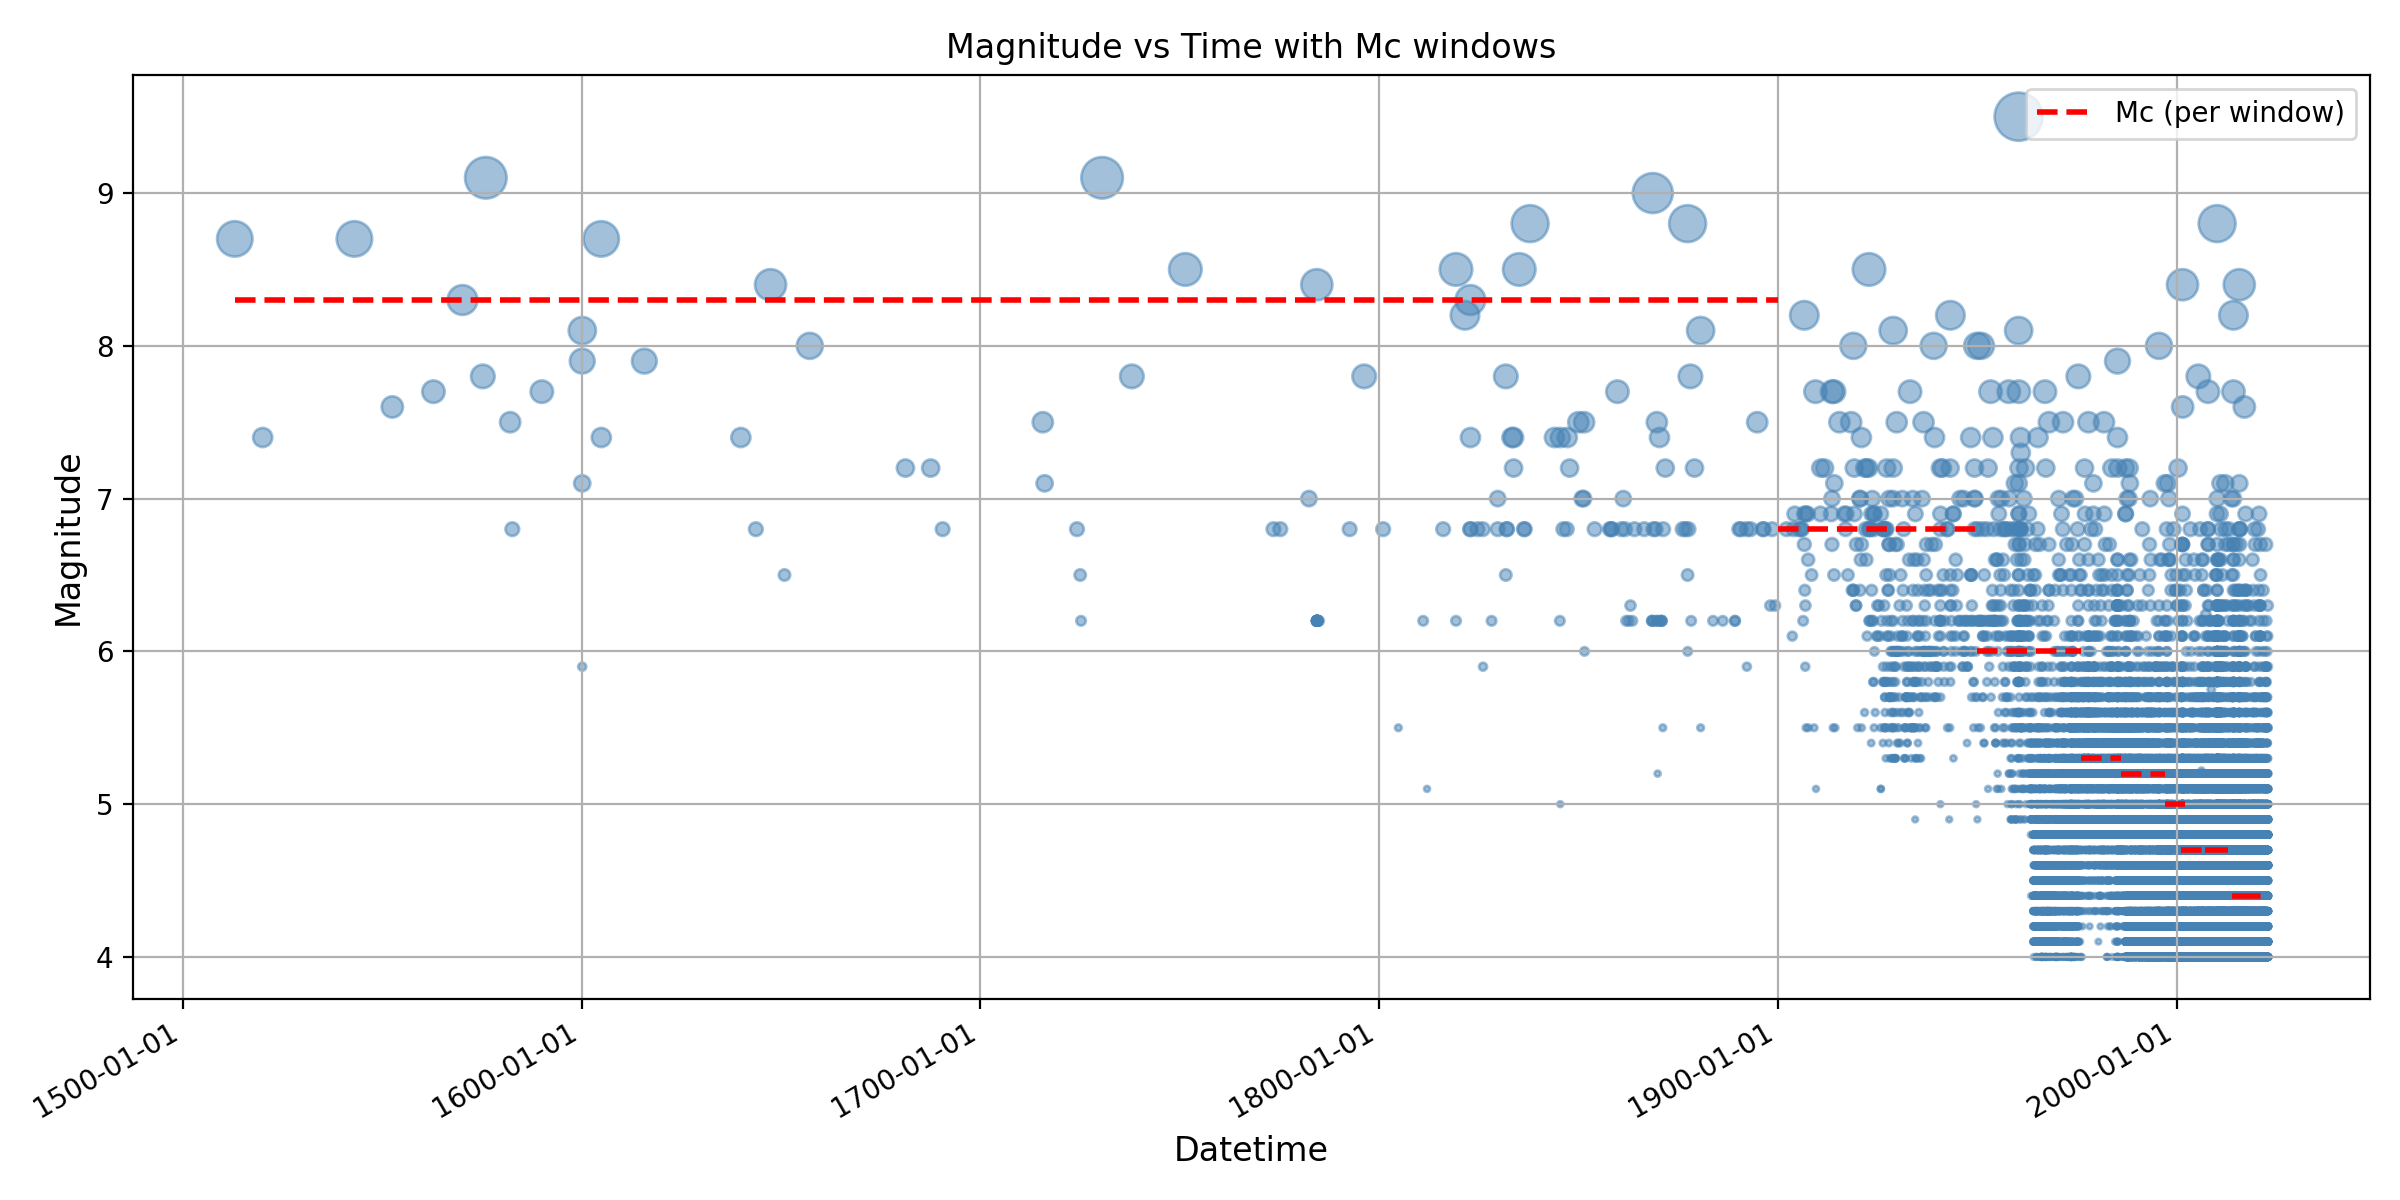
\includegraphics[width=0.6\textwidth]{./figures/mc}
		\end{figure}



\end{frame}

%}



\begin{frame}[t]
\frametitle{Construcción de un modelo de PSHA para Chile}

\begin{columns}[t]

	\column{.45\textwidth}
\textbf{Interfaz Subducción:}\\

	\vspace{0.5cm}

	\only<1>{
Un segmento:\\
Balance de momento geodético-sísmico
\begin{align*}
	\dot{M}^{\mathrm{seismic}}&=\chi\,\dot{M}_{s}^{\mathrm{geodetic}} \\
\dot{M}^{\mathrm{seismic}}(a,b,M_{\mathrm{c}})
&=
\int_{M_{\min}}^{\infty}
\lambda_{\mathrm{MFD}}(m)\,M_0(m)\,\mathrm{d}m \\
\dot{M}_{s}^{\mathrm{geodetic}}
&=
\mu\,A\,v
\end{align*}
{\footnotesize
\(\lambda(m)\): Seismicity rate for $m$ \\
\(M_c\): Corner-magnitude para Tapered TGR \\
\(\chi\): coef. coupling (0.83, Johnson et al., 2023, GEM) \\
\(\mu\): módulo de corte \\
\(A\): área de la zona bloqueada \\
\(v\): velocidad de convergencia.
}
}

	\only<2>{
	Multiples segmentos:\\
	Déficit de momento sísmico
\begin{align*}
\dot{M}^{\mathrm{def}}_i
&=
\chi\,\dot{M}_{s,i}^{\mathrm{geodetic}}
-
\dot{M}^{\mathrm{cat}}_i, \quad i = 1,\dots,N.
\end{align*}

{\footnotesize
\(\dot{M}^{\mathrm{def}}_i\): tasa de \textbf{déficit} de momento sísmico del segmento \(i\) \\
\(\dot{M}^{\mathrm{cat}}_i\): tasa de momento sísmico liberado en el catálogo \\
}

	}
		\column{.55\textwidth}
	\only<1>{
		\begin{figure}
		\vspace*{-1.cm}
		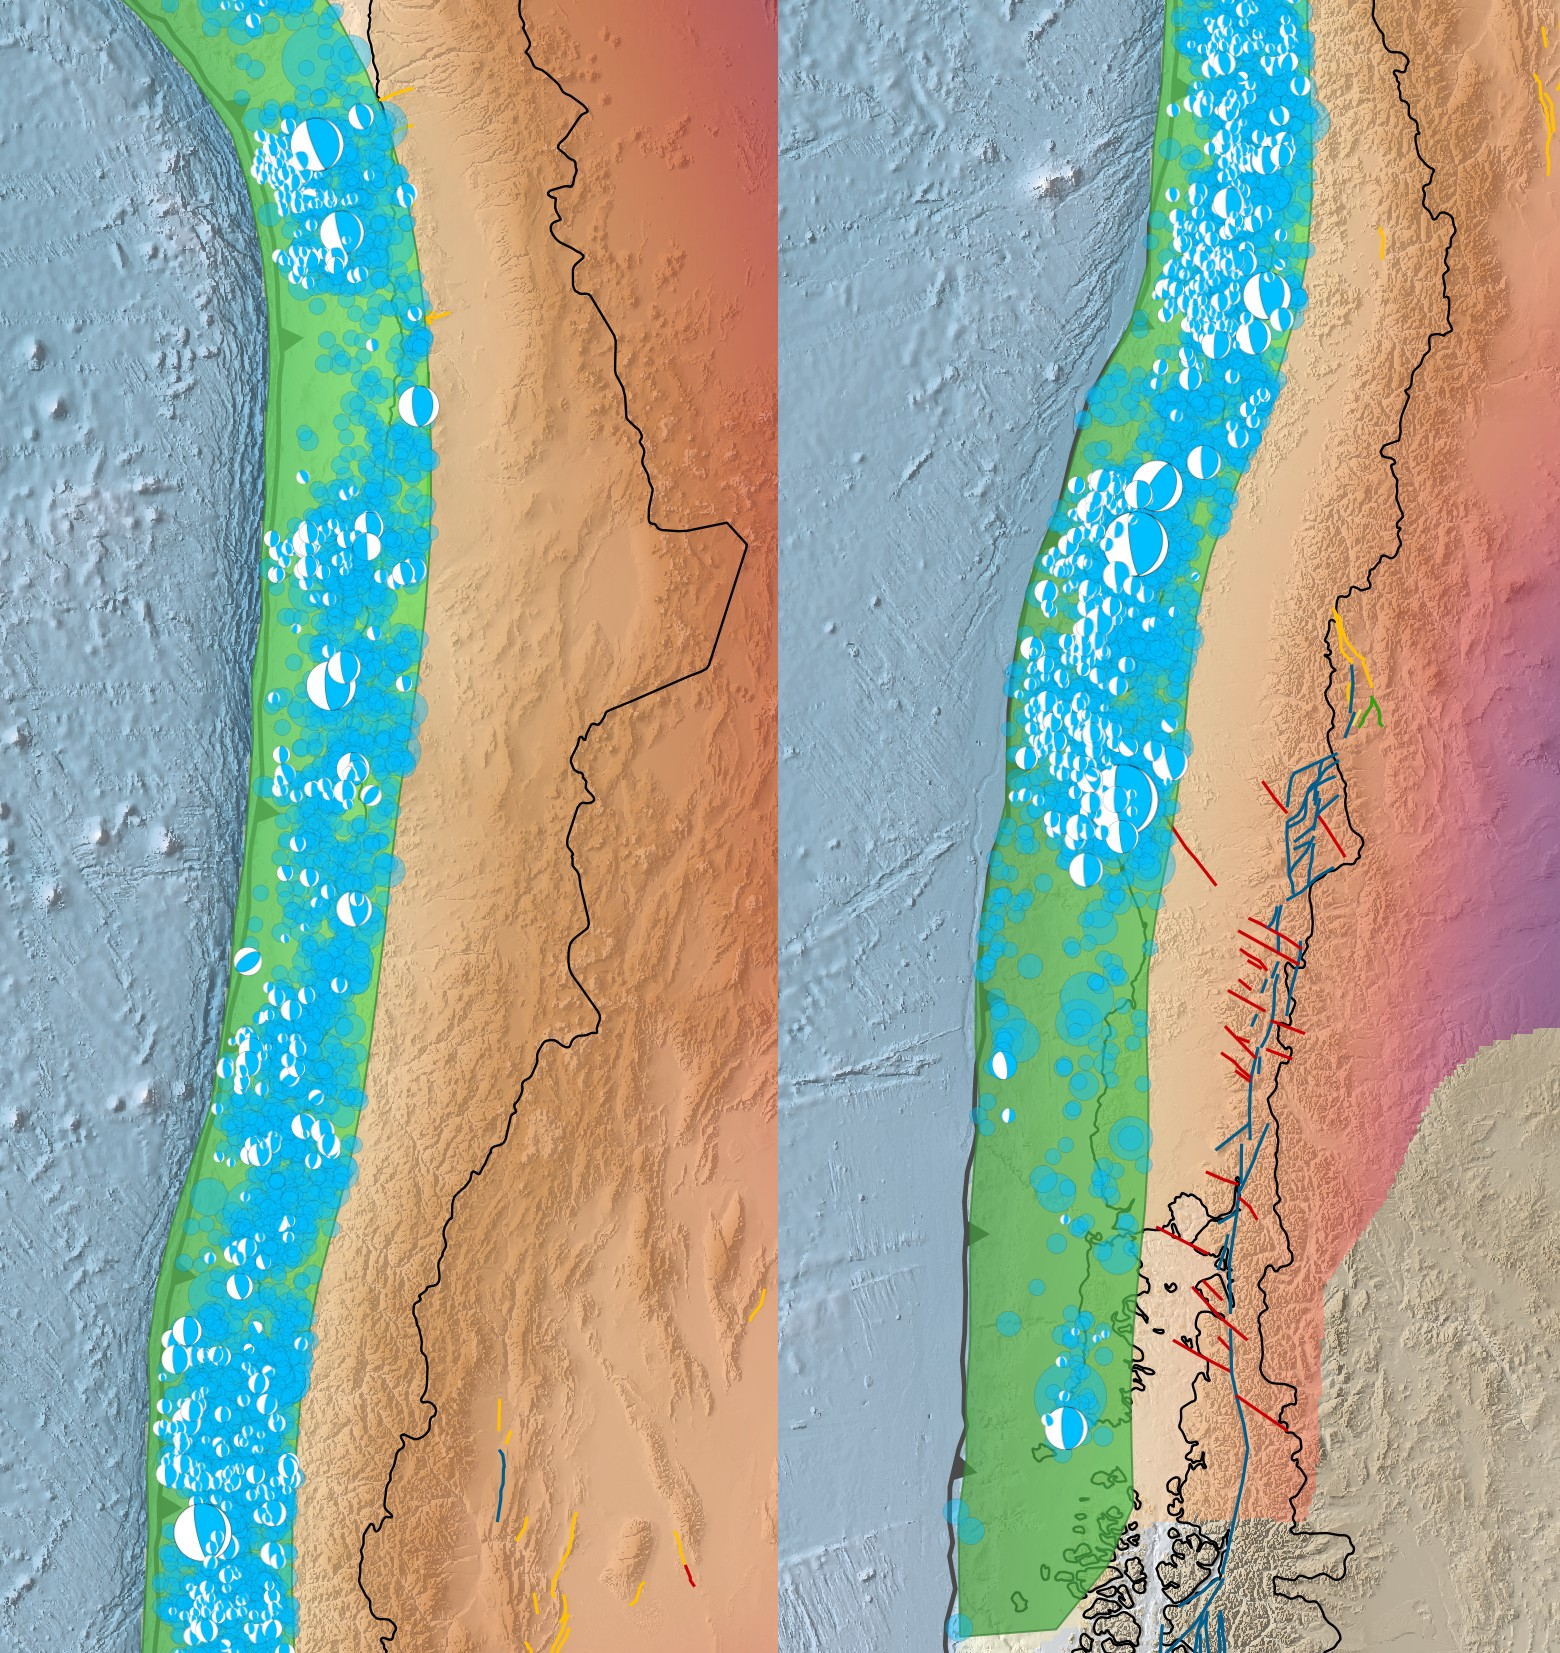
\includegraphics[width=0.85\textwidth]{./figures/sub_locked}
		\end{figure}
	}
	\only<2>{
		\begin{figure}
		\vspace*{-1.cm}
		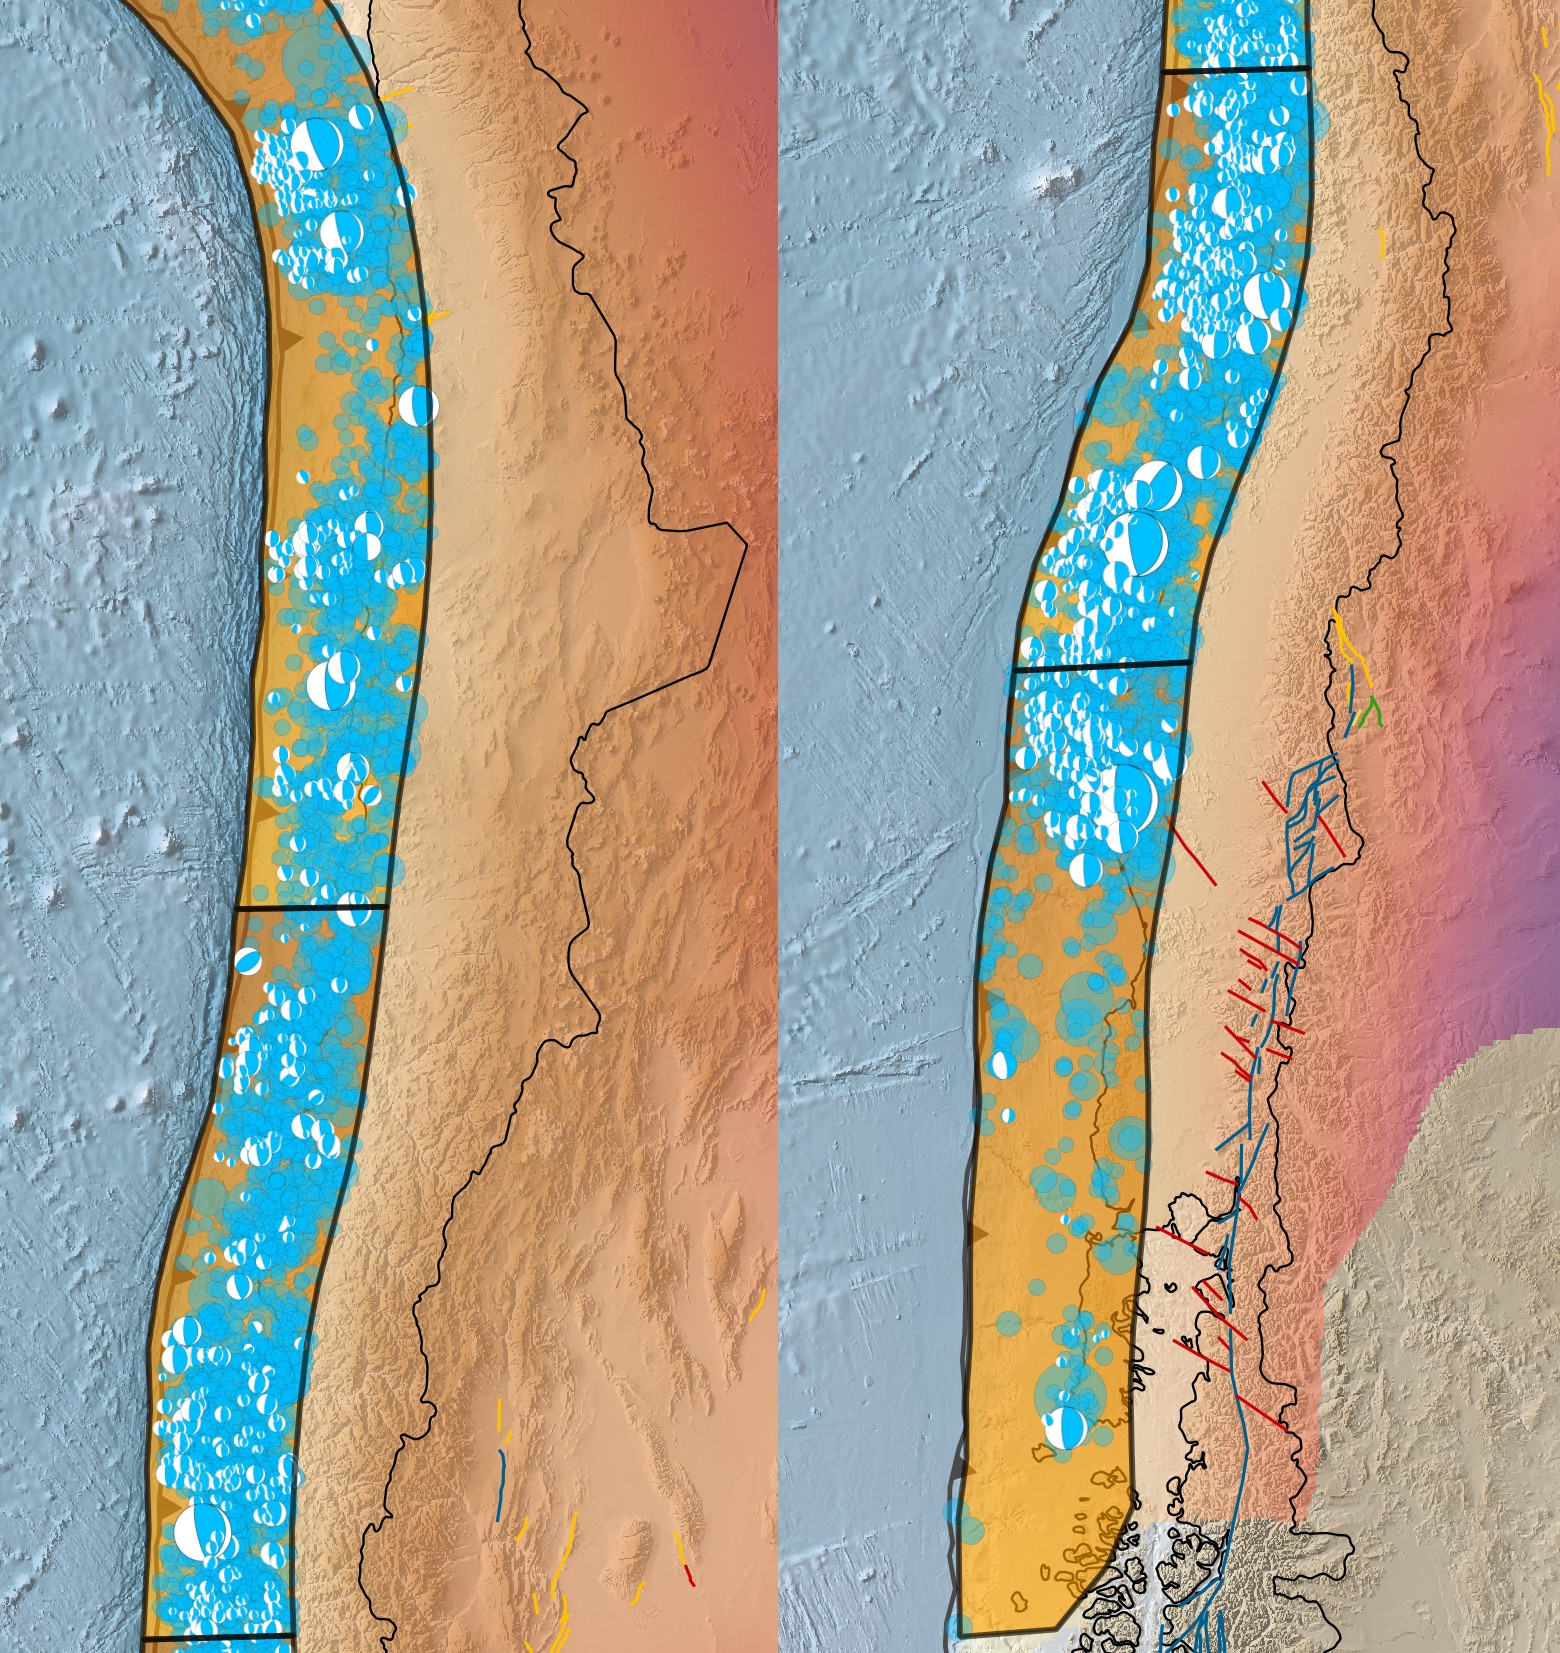
\includegraphics[width=0.85\textwidth]{./figures/sub_locked_seg}
		\end{figure}
	}
\end{columns}


\end{frame}

\begin{frame}[t]
\frametitle{Construcción de un modelo de PSHA para Chile}

\begin{columns}[t]

	\column{.45\textwidth}
\textbf{Subducción - Intra-placa}\\

	\begin{itemize}
		\item Adaptive Smoothed-Seismicity Model (Helmstetter et al., 2007)
		\item Truncated GR
		\item $b$-value del catalogo (van der Elst, 2023)
		\item $M_{max}$ del catálogo (+0.2)
		\item Resolver para $a$
	\end{itemize}


		\column{.55\textwidth}
	\only<1>{
		\begin{figure}
		\vspace*{-1.cm}
		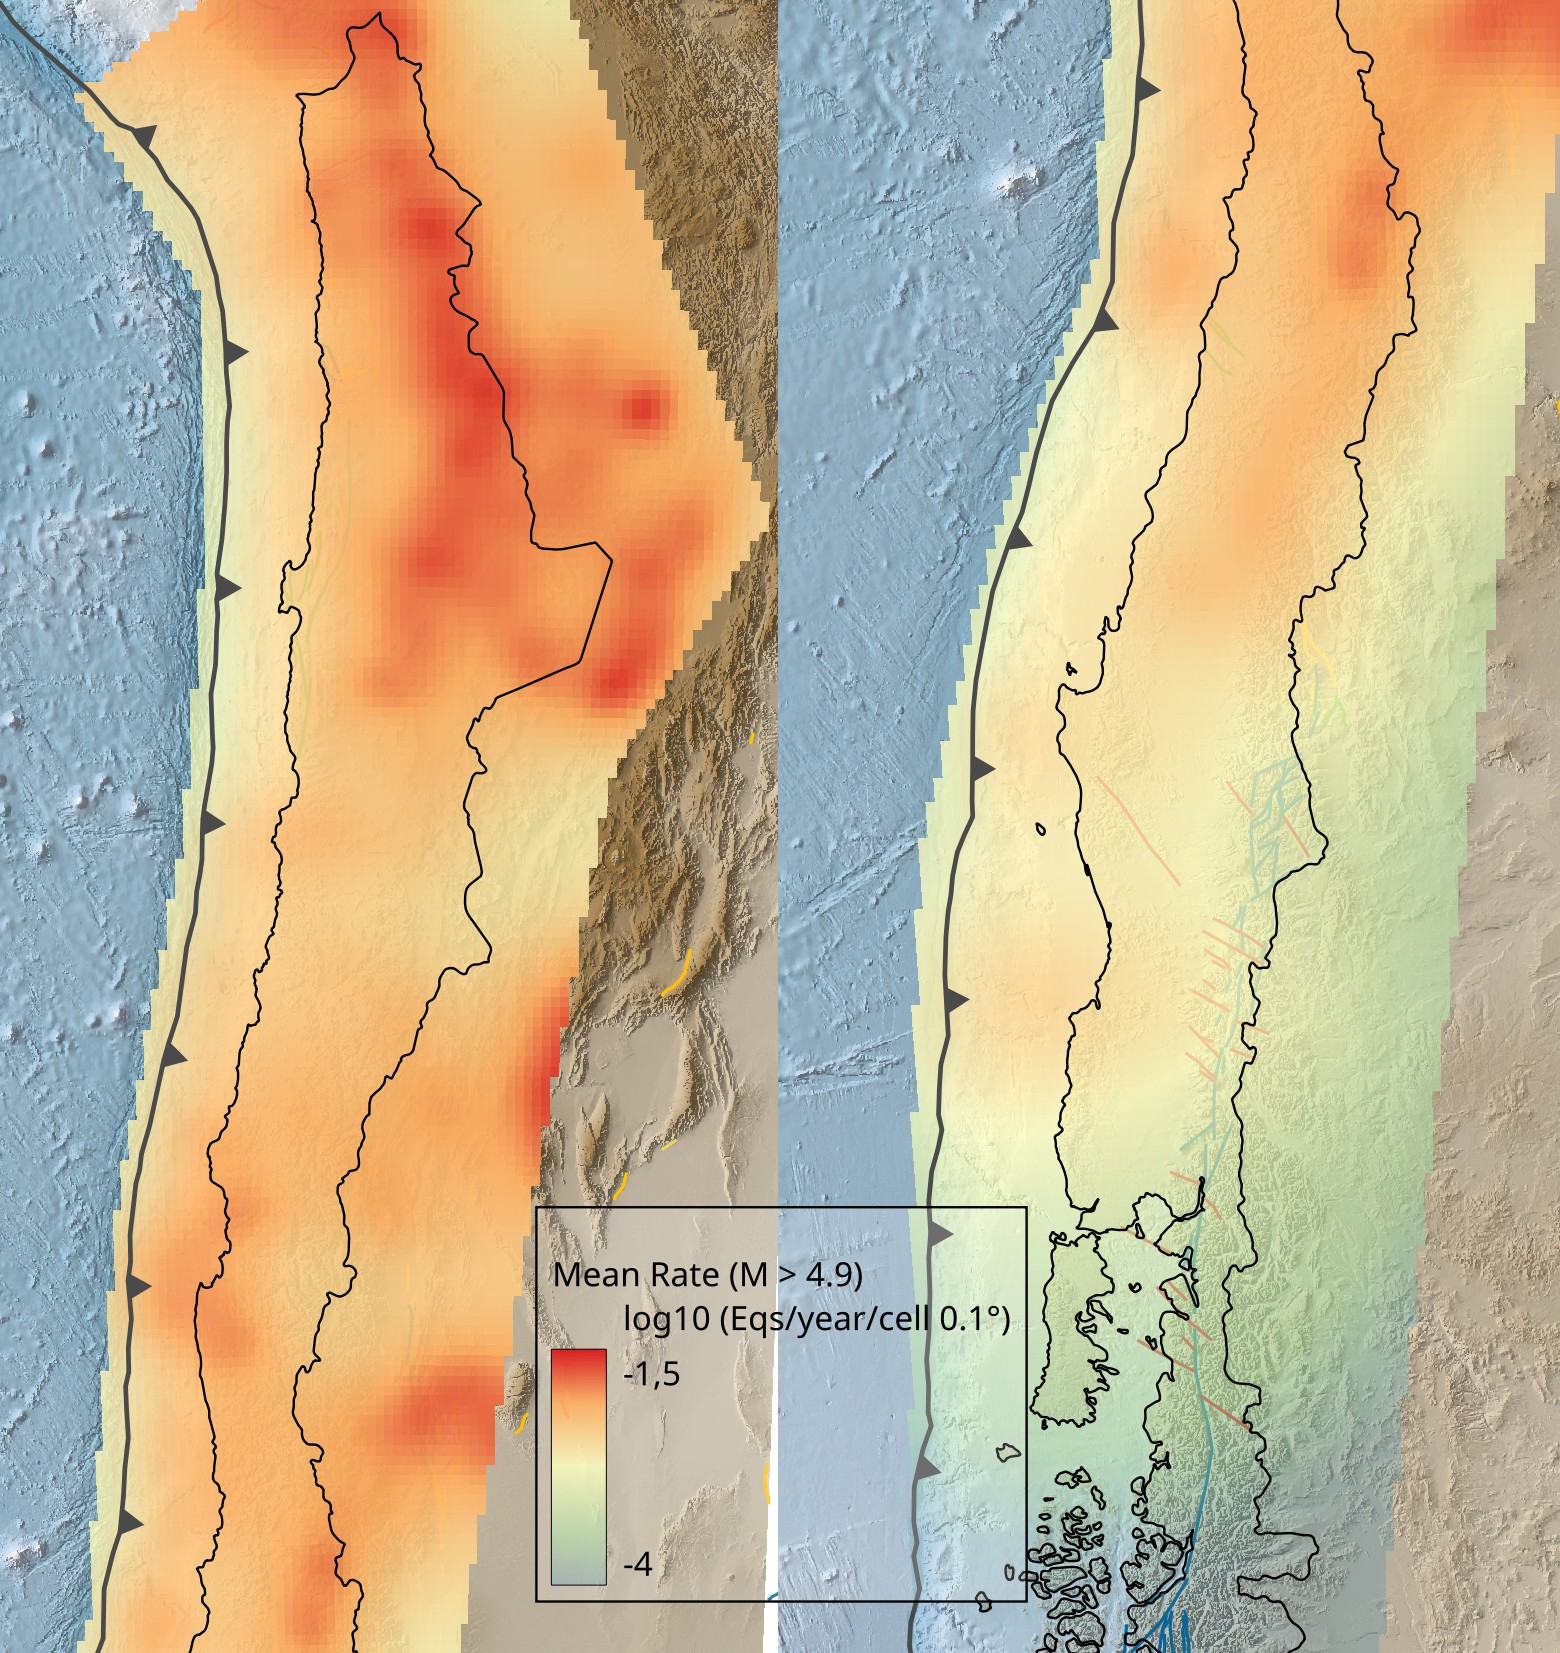
\includegraphics[width=0.85\textwidth]{./figures/forecast_intra}
		\end{figure}
	}
	\only<2>{
		\begin{figure}
		\vspace*{-1.cm}
		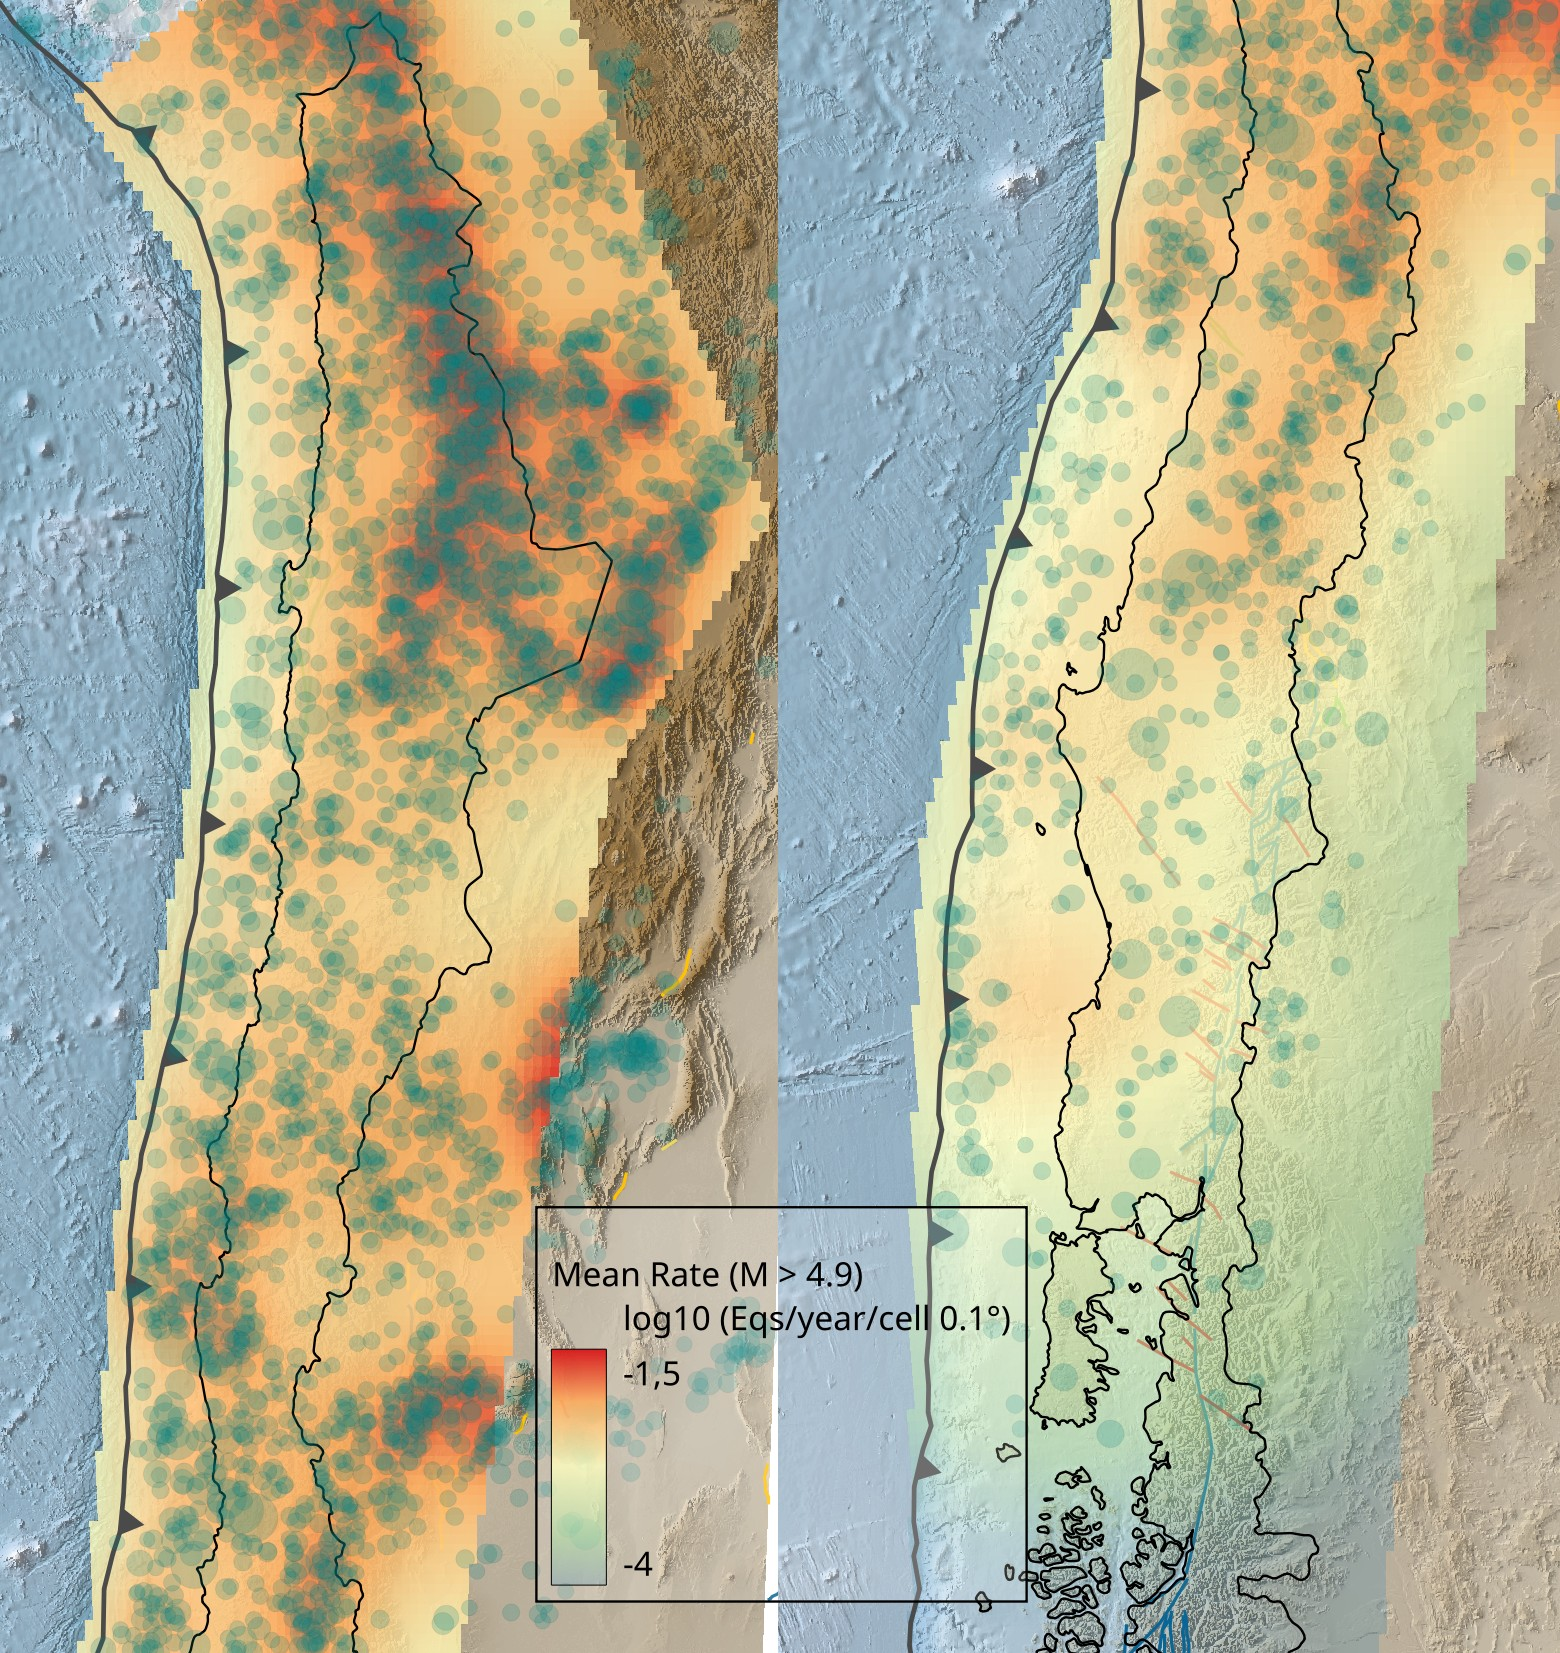
\includegraphics[width=0.85\textwidth]{./figures/forecast_intra_events}
		\end{figure}
	}
\end{columns}

\end{frame}


\begin{frame}[t]
	\frametitle{Construcción de un modelo de PSHA para Chile}

	\begin{columns}[t]

		\column{.45\textwidth}

			\textbf{Sismicidad Cortical}\\

	\begin{itemize}
		\item Adaptive Smoothed-Seismicity Model (Helmstetter et al., 2007)
		\item Truncated GR
		\item $b$-value del catalogo (van der Elst, 2023)
		\item $M_{max}$ del catálogo (+0.2)
		\item Resolver para $a$
	\end{itemize}

			\column{.55\textwidth}
		\only<1>{
			\begin{figure}
			\vspace*{-1.cm}
			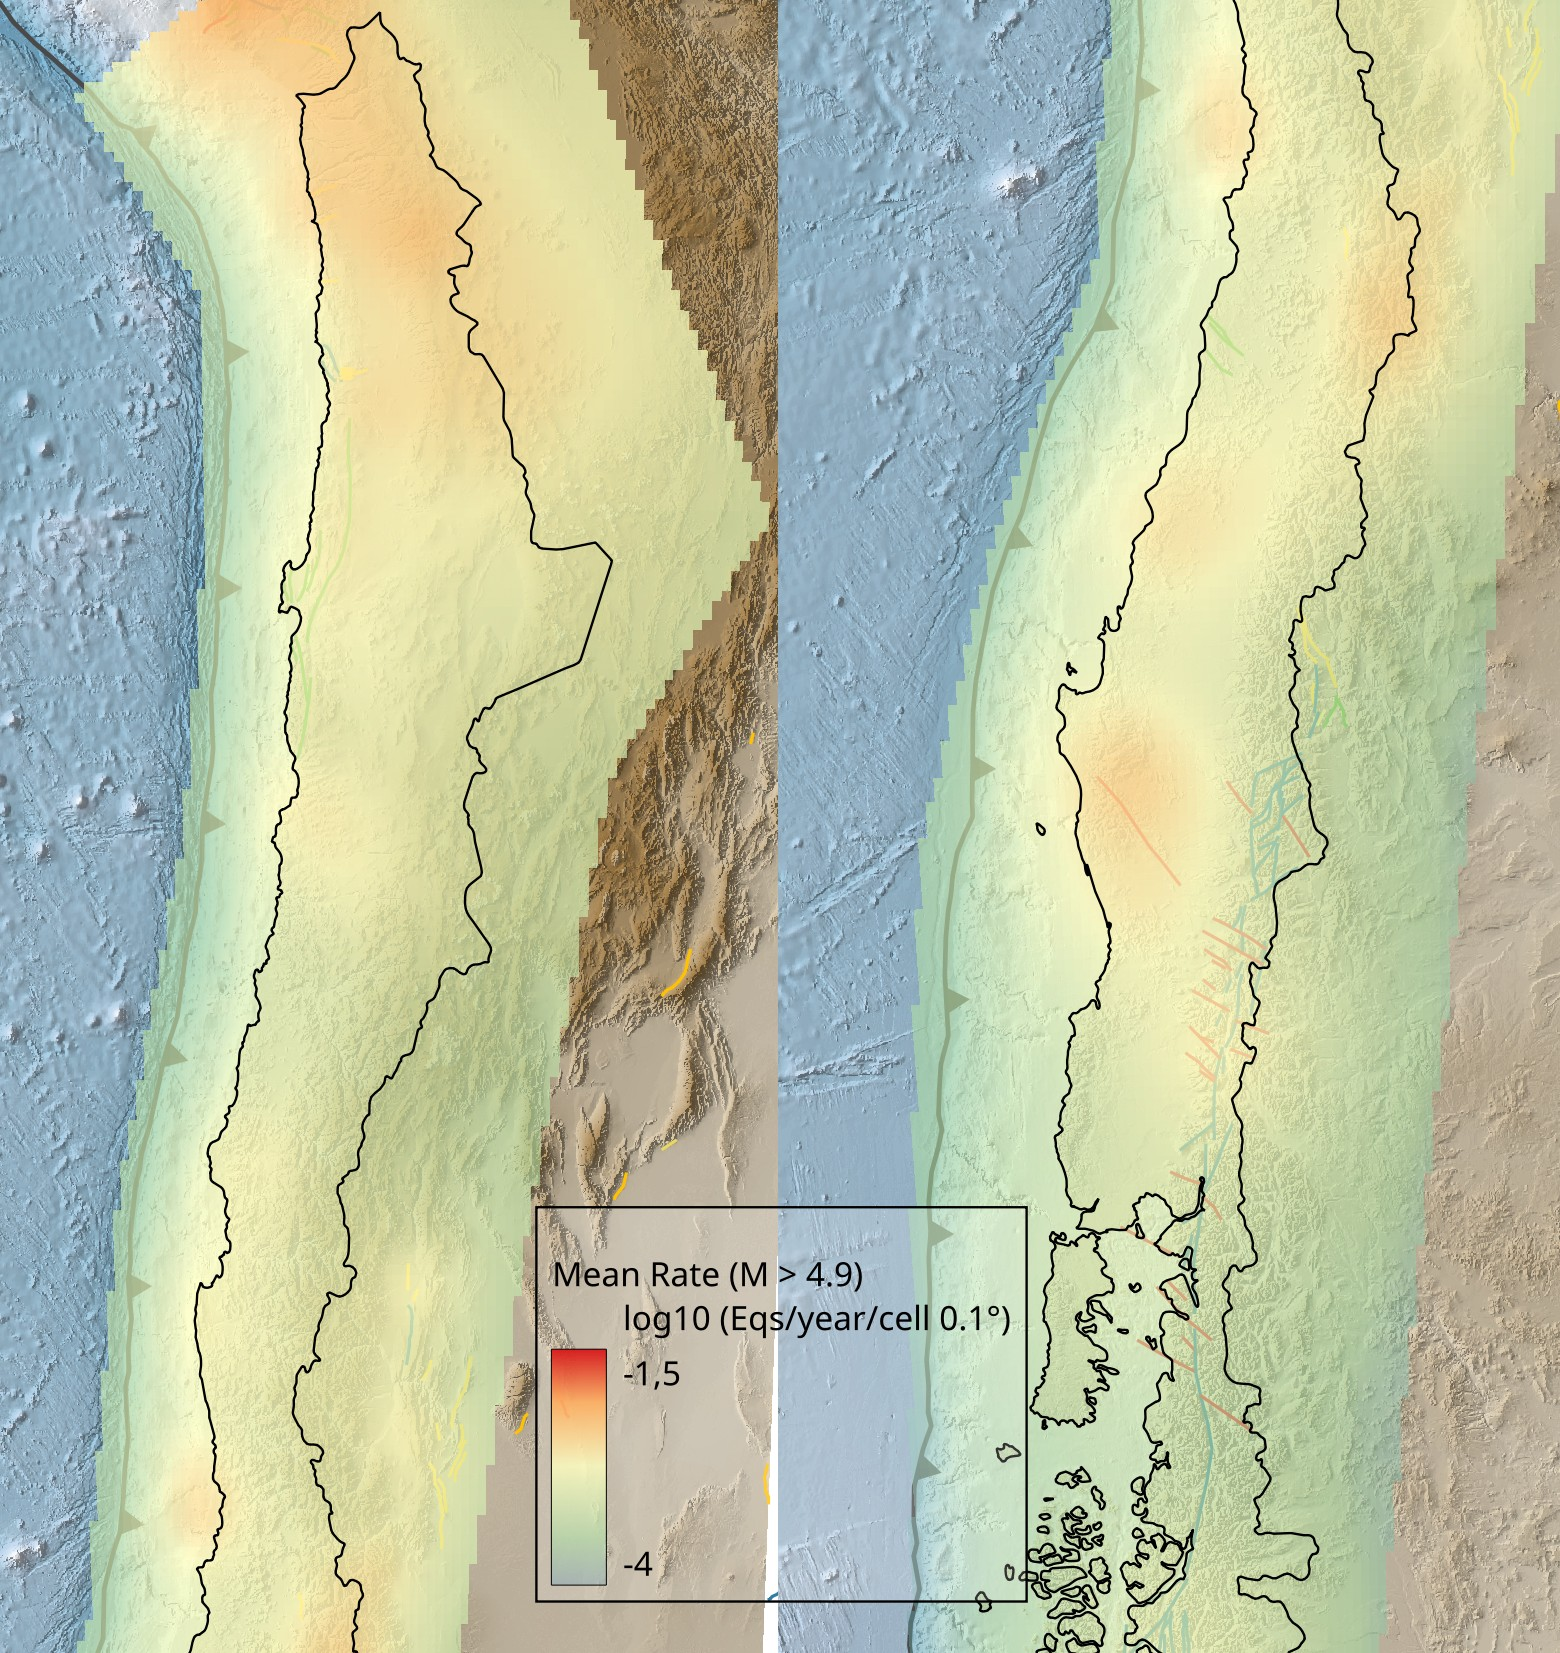
\includegraphics[width=0.85\textwidth]{./figures/forecast_crust}
			\end{figure}
		}
		\only<2>{
			\begin{figure}
			\vspace*{-1.cm}
			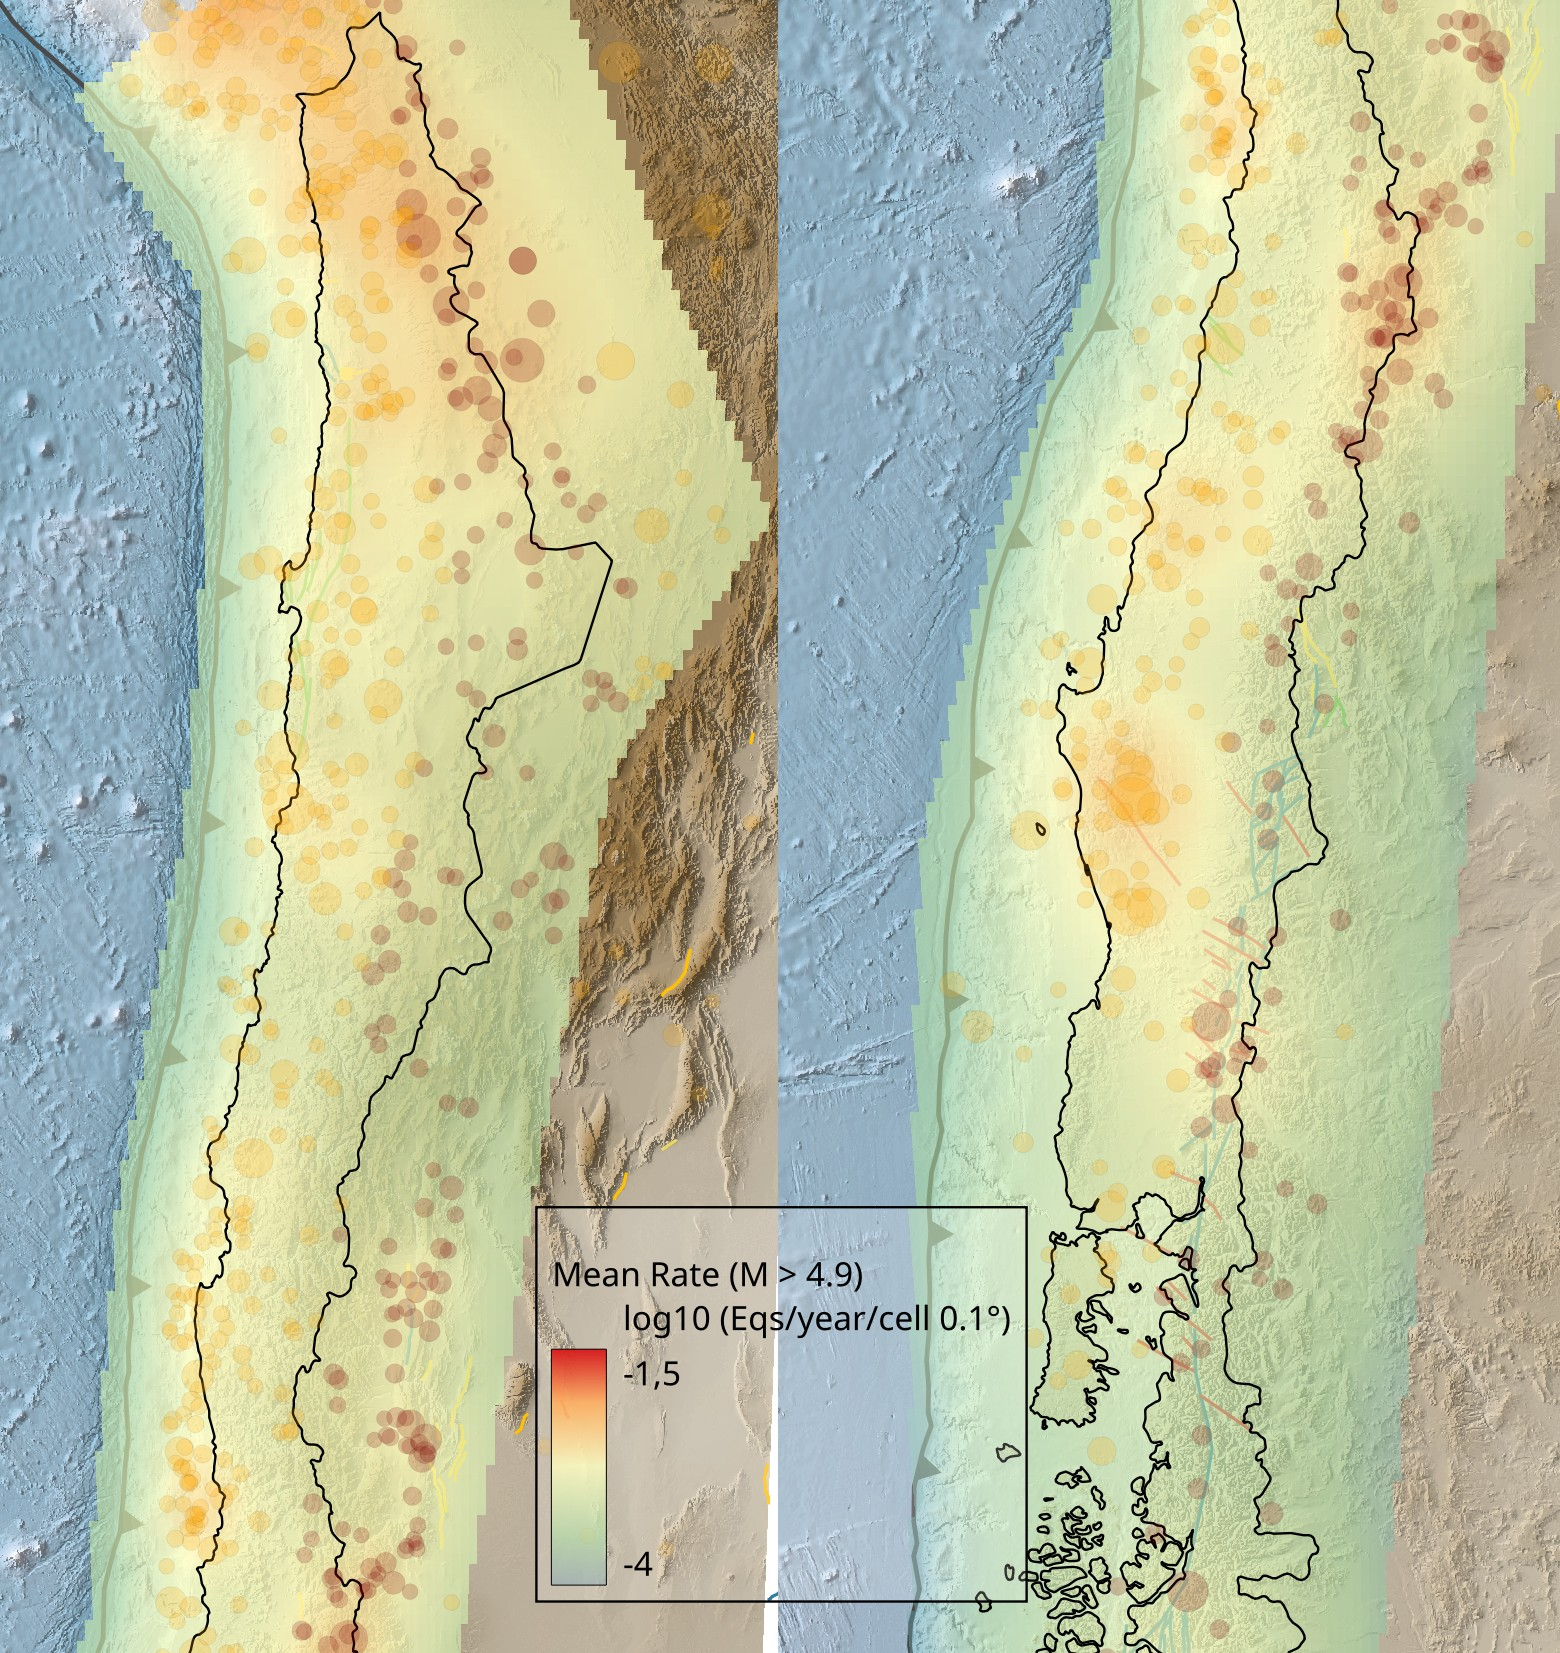
\includegraphics[width=0.85\textwidth]{./figures/forecast_crust_events}
			\end{figure}
		}
	\end{columns}

\end{frame}


\begin{frame}[t]
	\frametitle{Construcción de un modelo de PSHA para Chile}

	\begin{columns}[t]

		\column{.4\textwidth}

			\textbf{Fallas corticales}\\

	\begin{itemize}
		\item Truncated o Tapered GR
		\item $b$-value del catalogo (van der Elst, 2023)
		\item $M_{max}$ de la geometría o Santibańez et al., 2018
		\item Resolver para $a$
	\end{itemize}
\begin{align*}
	\dot{M}^{\text{long-term}} &= 	\dot{M}^{\mathrm{seismic}} \\
	\dot{M}^{\text{long-term}} &=
\phi\,\mu\,L\,W\,\dot{s}_r
\end{align*}

		Donde $\dot{s}_r$ es el slip rate y $\phi$ el factor sísmico-asísmico. Asumimos $\phi_i=[0.5, 0.75, 1]$
		con pesos $w_i=[0.25, 0.5, 0.25]$
			\column{.6\textwidth}


			\begin{figure}

			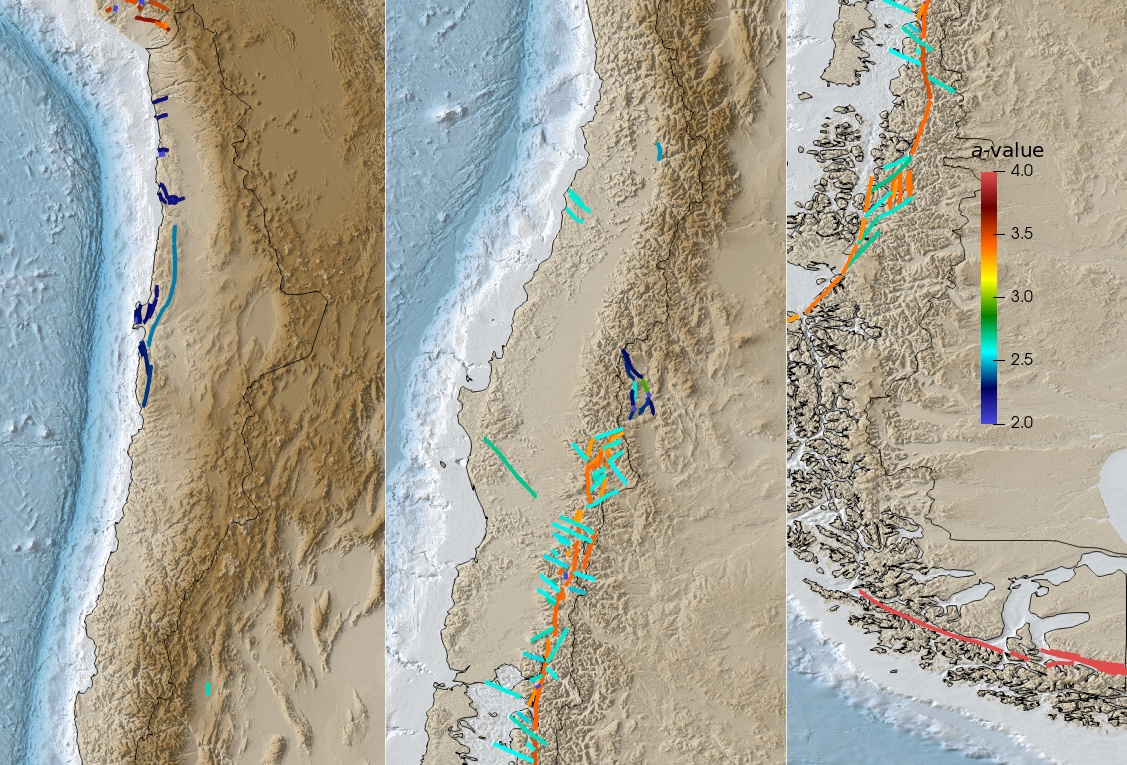
\includegraphics[width=0.95\textwidth]{./figures/a_val_faults}
			\end{figure}

	\end{columns}

\end{frame}

\begin{frame}[t]
	\frametitle{Mapa de Amenaza Sísmica}

	\only<1>{
			\begin{figure}
			\vspace*{-0.3cm}
			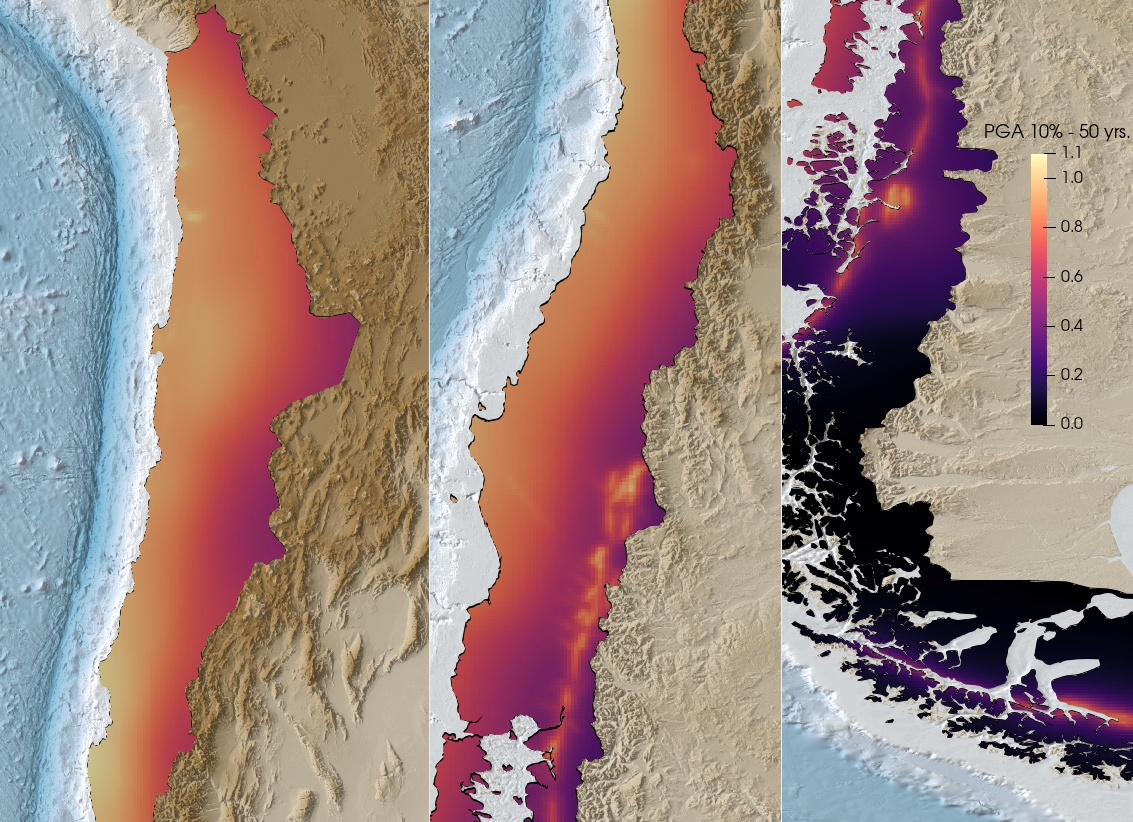
\includegraphics[width=0.62\textwidth]{./figures/hazardmap_faults}
				\caption*{Mapa de amenaza \textbf{considerando} fallas corticales: PGA con un 10\% de exceedencia en 50 años , $V_{\mathrm{S}30}=250 \, \mathrm{m}/\mathrm{s}$. Cálculos hechos con openquake (Pagani et al., 2012)}
			\end{figure}
	}
	\only<2>{
			\begin{figure}
			\vspace*{-0.3cm}
			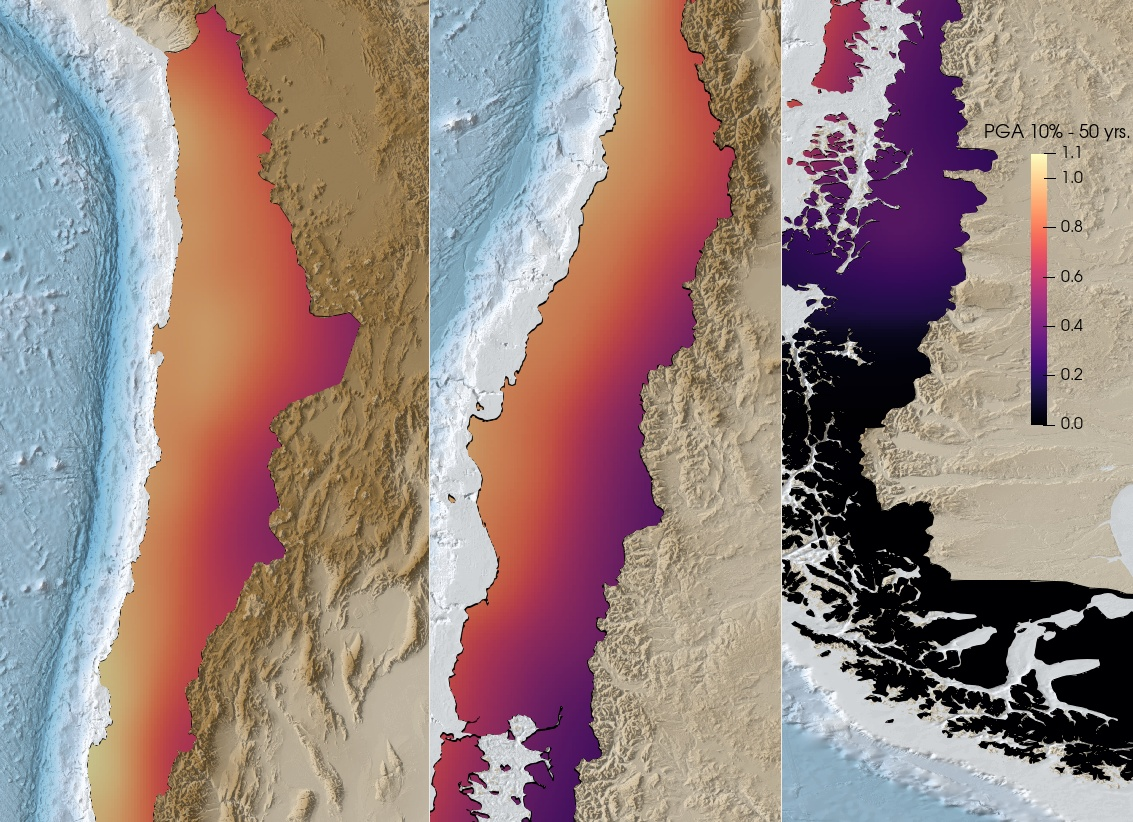
\includegraphics[width=0.62\textwidth]{./figures/hazardmap_nofaults}
			\caption*{Mapa de amenaza \textbf{excluyendo} fallas corticales: PGA con un 10\% de exceedencia en 50 años, $V_{\mathrm{S}30}=250 \, \mathrm{m}/\mathrm{s}$. Cálculos hechos con openquake (Pagani et al., 2012)}
			\end{figure}
	}
	\only<3>{
				\begin{figure}
			\vspace*{-0.3cm}
			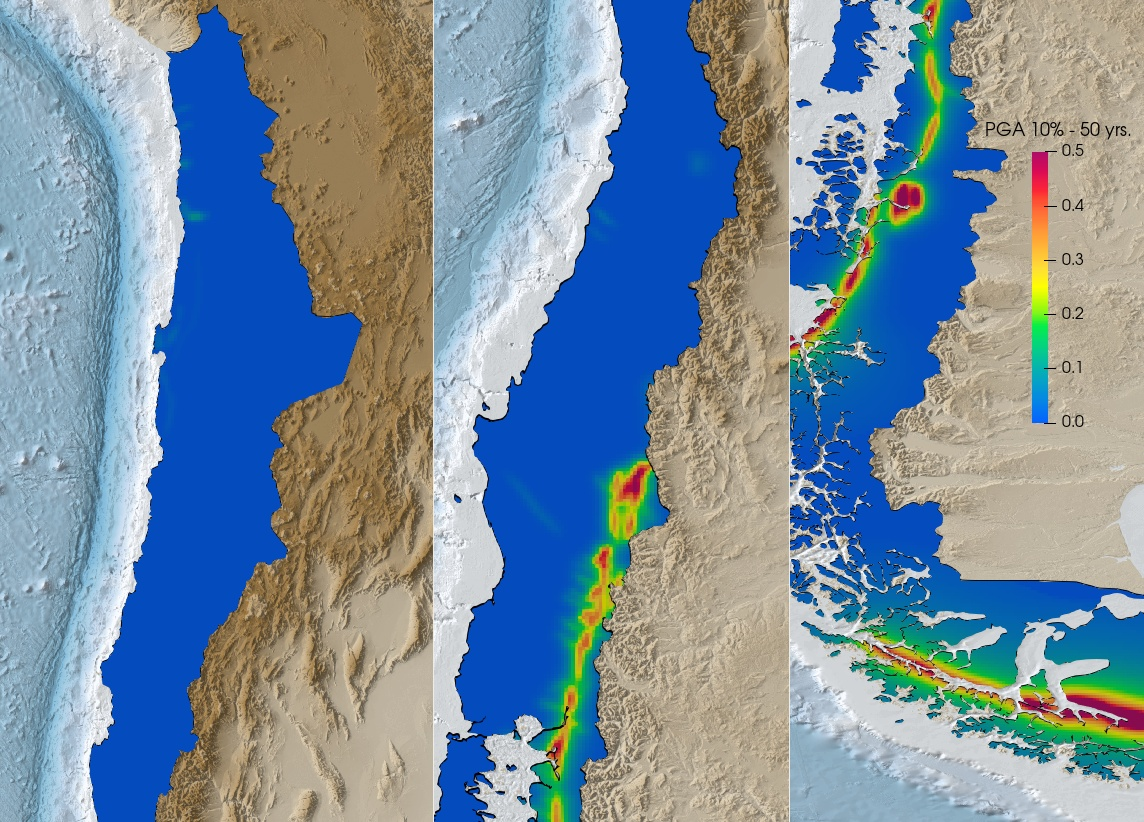
\includegraphics[width=0.62\textwidth]{./figures/hazardmap_absdiff}
				\caption*{Diferencia absoluta entre mapas con y sin fallas corticales.}
			\end{figure}
	}
		\only<4>{
				\begin{figure}
			\vspace*{-0.3cm}
			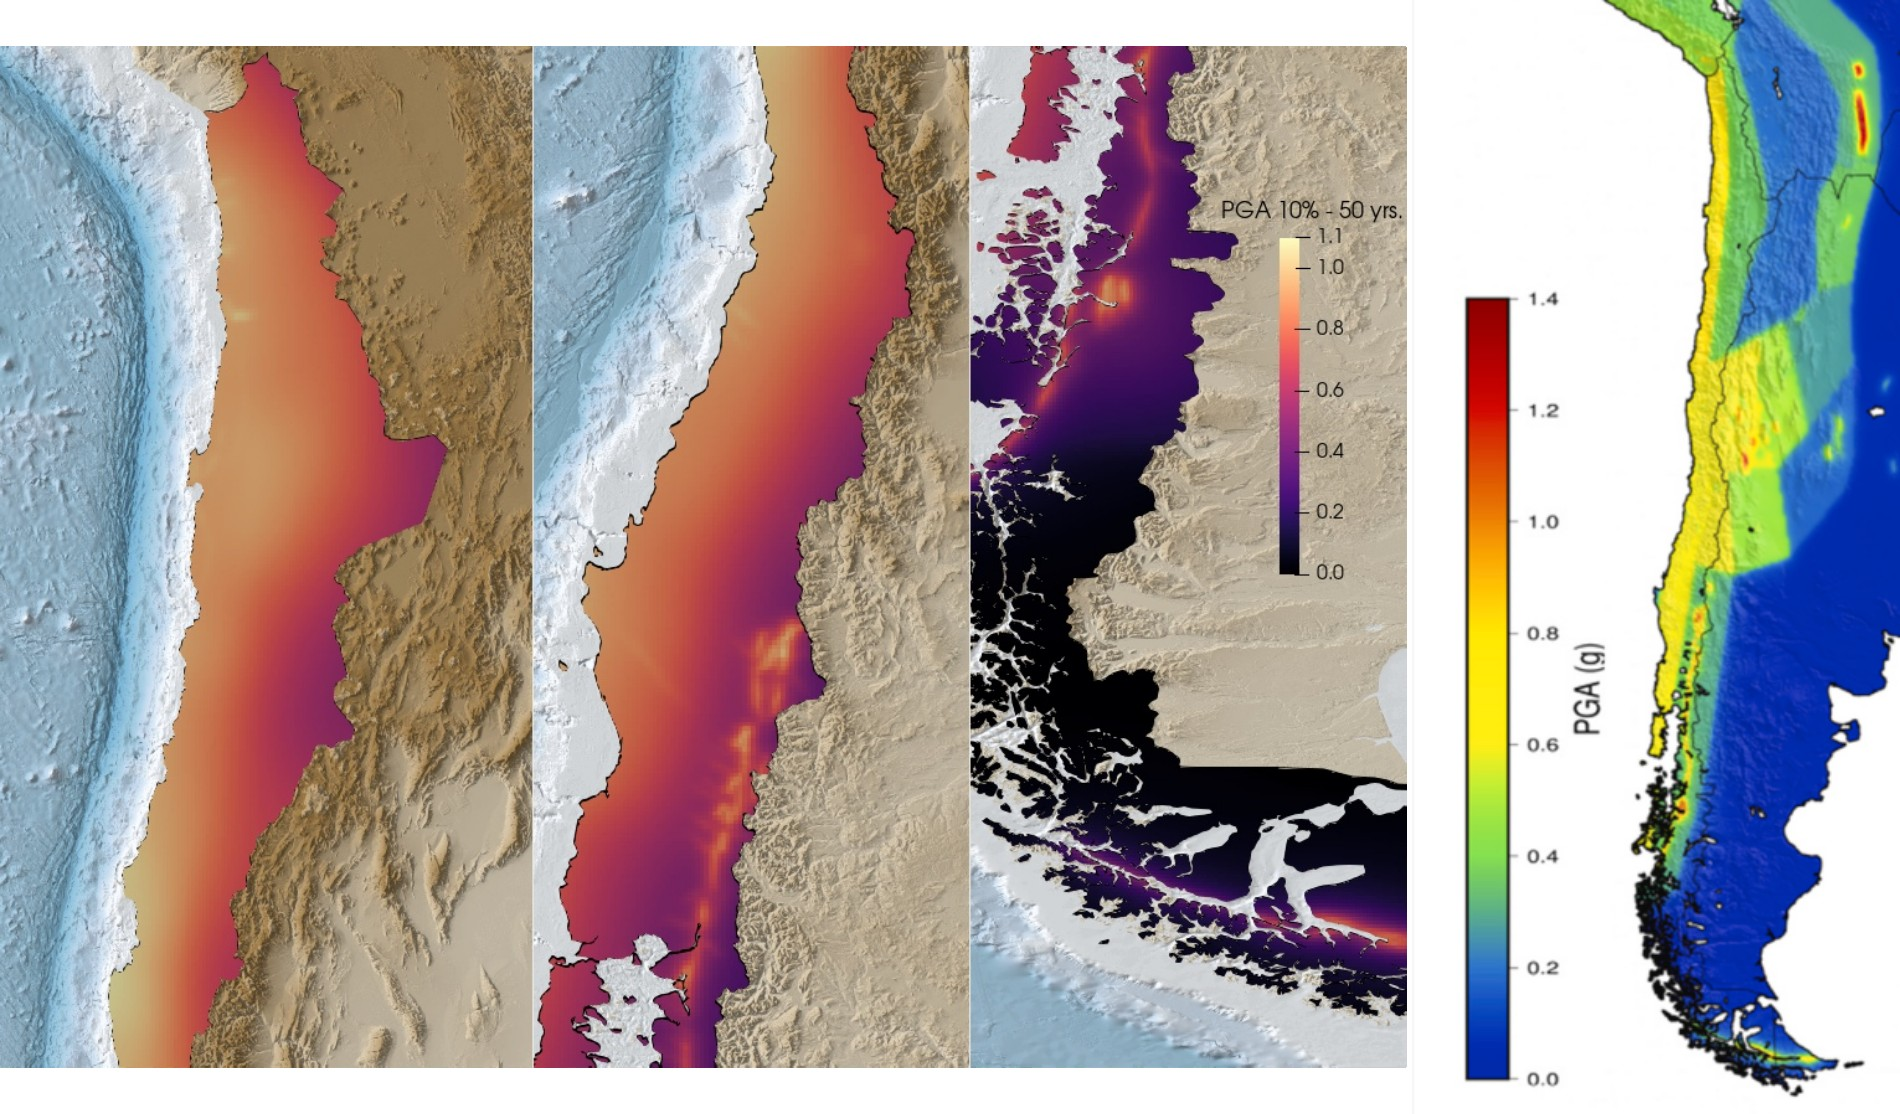
\includegraphics[width=0.75\textwidth]{./figures/comp}
				\caption*{Comparación con modelo de referencia SARA/GEM (Costa et al., 2020)}
			\end{figure}
	}
\end{frame}

	\begin{frame}[t]
	\frametitle{Curvas de Amenaza Sísmica}

	\only<1>{
			\begin{figure}
			\vspace*{-0.3cm}
			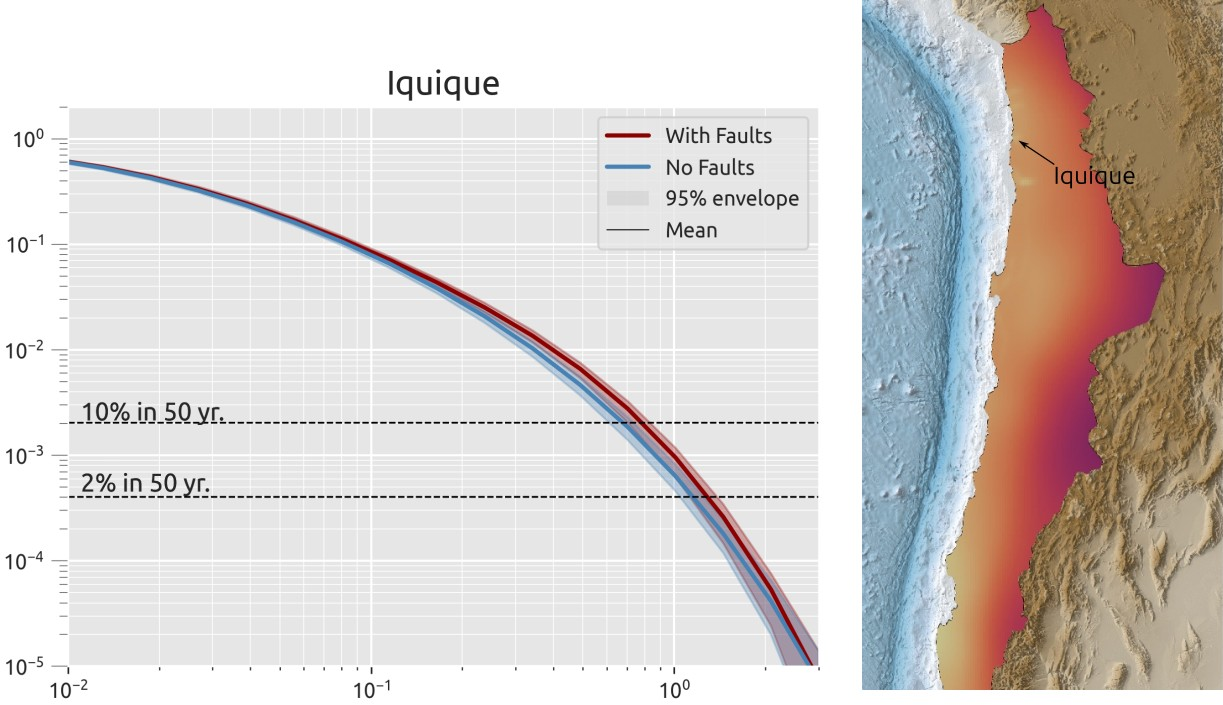
\includegraphics[width=0.72\textwidth]{./figures/curva_iquique}
				\caption*{Curva de amaneaza sísmica para modelos con y sin fallas corticales ($V_{\mathrm{S}30}=250 \, \mathrm{m}/\mathrm{s}$).}
			\end{figure}
	}
	\only<2>{
			\begin{figure}
			\vspace*{-0.3cm}
			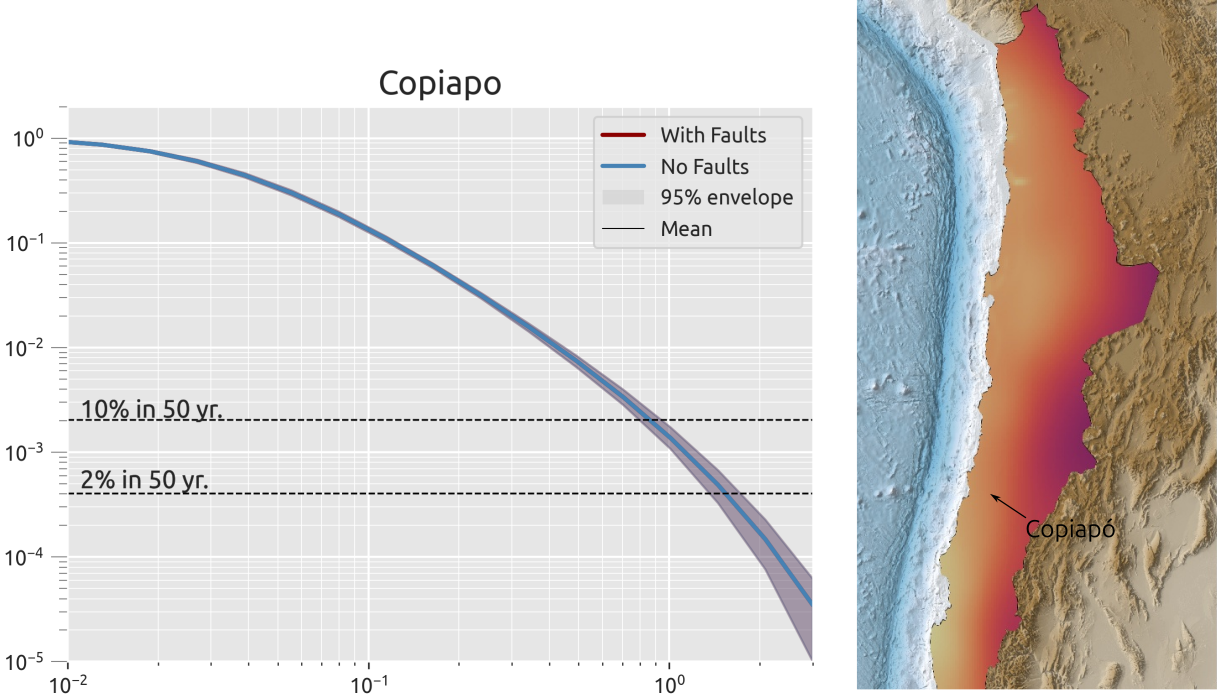
\includegraphics[width=0.72\textwidth]{./figures/curva_cupiapo}
			\caption*{Curva de amaneaza sísmica para modelos con y sin fallas corticales ($V_{\mathrm{S}30}=250 \, \mathrm{m}/\mathrm{s}$).}
			\end{figure}
	}
	\only<3>{
				\begin{figure}
			\vspace*{-0.3cm}
			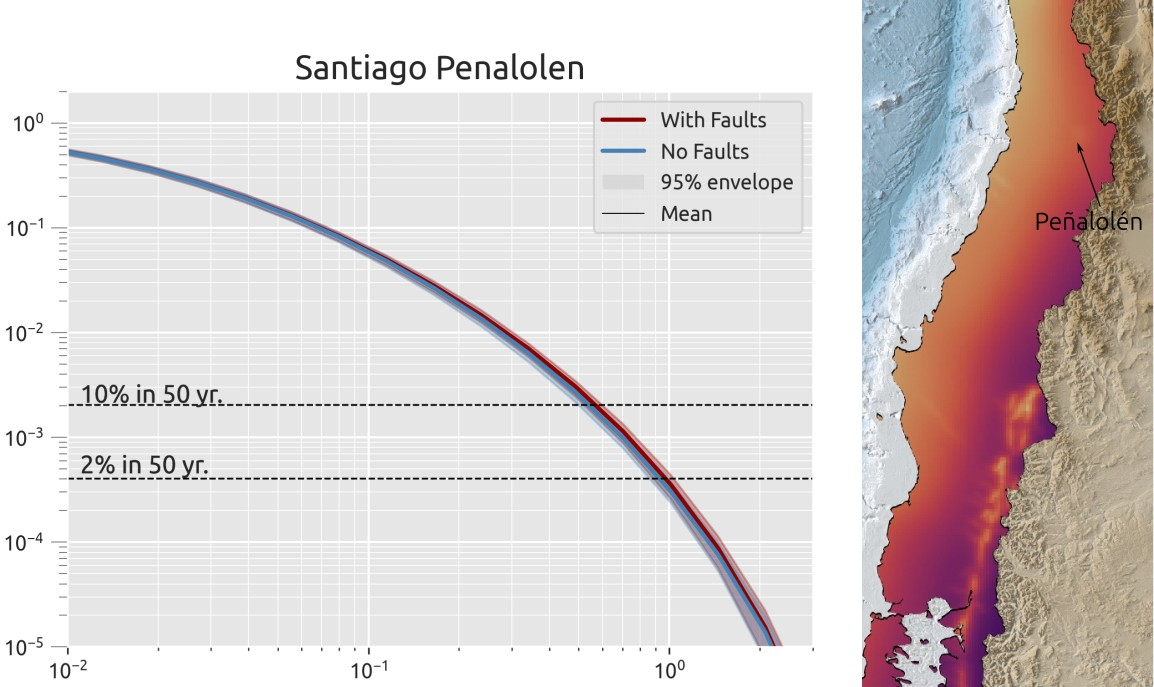
\includegraphics[width=0.72\textwidth]{./figures/curva_santiago}
				\caption*{Curva de amaneaza sísmica para modelos con y sin fallas corticales ($V_{\mathrm{S}30}=250 \, \mathrm{m}/\mathrm{s}$).}
			\end{figure}
	}
	\only<4>{
		\begin{figure}
	\vspace*{-0.3cm}
	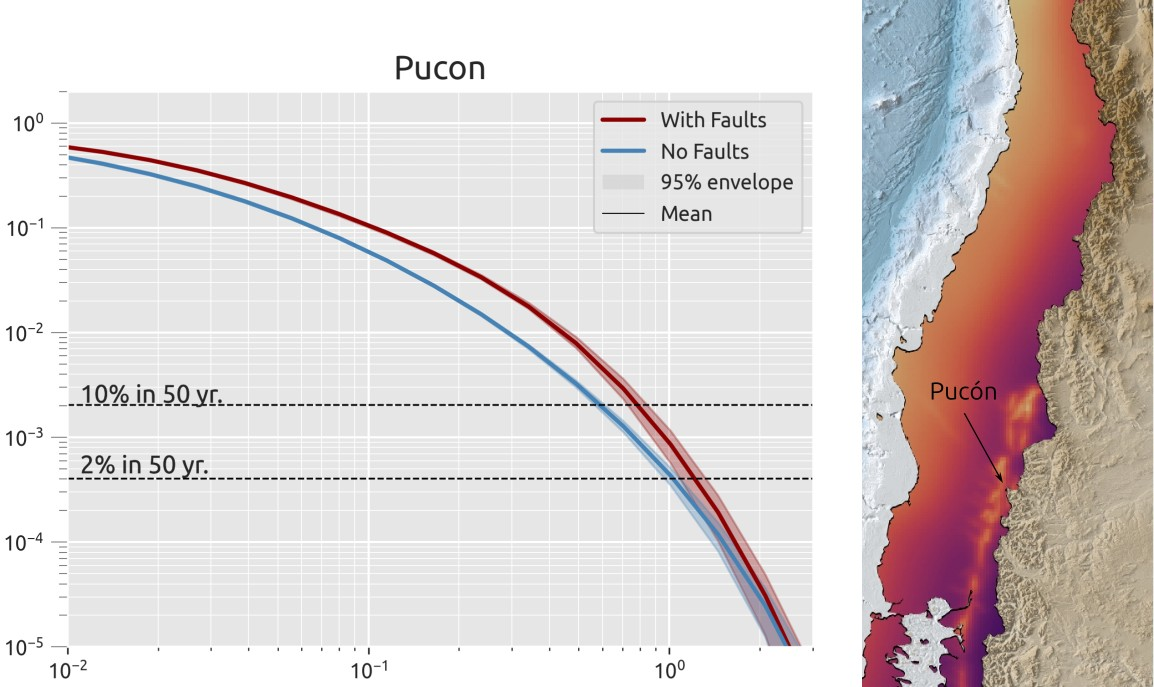
\includegraphics[width=0.72\textwidth]{./figures/curva_pucon}
		\caption*{Curva de amaneaza sísmica para modelos con y sin fallas corticales ($V_{\mathrm{S}30}=250 \, \mathrm{m}/\mathrm{s}$).}
	\end{figure}
}
\end{frame}



\begin{frame}[t]\frametitle{Discusión}


\begin{itemize}
  \item Construimos un modelo base y sencillo de peligro sísmico para Chile,
        para evaluar el impacto relativo de las fallas corticales
        frente a otras fuentes.

  \item El modelo se implementó con código modular y abierto, siguiendo
        principios FAIR, de forma que las supuestos puedan
        reproducirse, rastrearse y modificarse.

  \item El impacto de las fallas corticales es, en muchos casos, comparable
        al intervalo de confianza de la subducción, pero en otros excede
        significativamente el hazard de subducción (p.ej. diferencias
        mayores a $\sim 0.2$g en PGA).

  \item El \emph{slip rate} es uno parámetros clave: por
        encima de cierto umbral las fallas pueden dominar localmente el
        peligro. Para nuestro modelo se necesita caracterizar
        mejor las fallas conocidas (incluyendo nuevos mapeos, p.ej.\ Marga--Marga), pero también entender
        su partición sísmica/asísmica.

  \item El impacto de las fallas corticales es espacialmente acotado y
        suele concentrarse en periodos de recurrencia cortos, lo que es
        especialmente relevante para diseño estructural residencial, microzonificación
        local y cálculos de riesgo.
\end{itemize}

\end{frame}


\begin{frame}[t]\frametitle{Conclusiones y perspectivas}

\begin{itemize}
  \item A pesar de usar metodos de otros modelos nacionales
        (p.ej.\ ESHM20 en Europa, esquemas de Nueva Zelanda), existen
        importantes limitaciones: modelación de la subducción, dependencia
        temporal, rupturas multi–segmento y evitar \emph{double counting}.

  \item Existe espacio para explorar nuevos desarrollos, como generar conjuntos de rupturas probabilísticas (UCERF3; Nueva Zelanda) o incluir catálogos sintéticos con modelos físicos para representar rupturas más complejas.

  \item Para fallas donde el hazard es bajo, efectos no
        considerados (near–fault, directividad, desplazamiento
        en superficie) podrían aumentar significativamente la amenaza,
        especialmente en aceleraciones espectrales altas.

  \item Los GMM son igual de relevantes que la
        caracterización de fuentes. Planeamos obtener factores de amplificación a escala regional (Weatherill et al., 2022) incorporando data, geología y pendiente.
\item Es crítico preparar el testing del rendimiento del modelo, usando alternatives open-source como floatcsep (Iturrieta et al., 2025, submitted JOSS) o eGsim (Zacarelli et al., 2024)

  \item El marco modular y abierto permite incorporar progresivamente
        nueva información de fallas, mejoras en la modelación de
        subducción y de ground motion, avanzando desde este modelo base
        hacia versiones mejor justificadas.

\end{itemize}

\end{frame}


\end{document}